\documentclass[12pt,spanish,oneside]{book}
\usepackage{lmodern}
\usepackage{amssymb,amsmath}
\usepackage{ifxetex,ifluatex}
\usepackage{fixltx2e} % provides \textsubscript
\ifnum 0\ifxetex 1\fi\ifluatex 1\fi=0 % if pdftex
  \usepackage[T1]{fontenc}
  \usepackage[utf8]{inputenc}
\else % if luatex or xelatex
  \ifxetex
    \usepackage{mathspec}
  \else
    \usepackage{fontspec}
  \fi
  \defaultfontfeatures{Ligatures=TeX,Scale=MatchLowercase}
\fi
% use upquote if available, for straight quotes in verbatim environments
\IfFileExists{upquote.sty}{\usepackage{upquote}}{}
% use microtype if available
\IfFileExists{microtype.sty}{%
\usepackage{microtype}
\UseMicrotypeSet[protrusion]{basicmath} % disable protrusion for tt fonts
}{}
\usepackage[inner = 3cm, outer = 2cm, top = 2.5cm, bottom = 2.5cm]{geometry}
\usepackage{hyperref}
\hypersetup{unicode=true,
            pdftitle={Tesis de Licenciatura},
            pdfauthor={Paola Corrales},
            pdfborder={0 0 0},
            breaklinks=true}
\urlstyle{same}  % don't use monospace font for urls
\ifnum 0\ifxetex 1\fi\ifluatex 1\fi=0 % if pdftex
  \usepackage[shorthands=off,main=spanish]{babel}
\else
  \usepackage{polyglossia}
  \setmainlanguage[]{spanish}
\fi
\usepackage{longtable,booktabs}
\usepackage{graphicx,grffile}
\makeatletter
\def\maxwidth{\ifdim\Gin@nat@width>\linewidth\linewidth\else\Gin@nat@width\fi}
\def\maxheight{\ifdim\Gin@nat@height>\textheight\textheight\else\Gin@nat@height\fi}
\makeatother
% Scale images if necessary, so that they will not overflow the page
% margins by default, and it is still possible to overwrite the defaults
% using explicit options in \includegraphics[width, height, ...]{}
\setkeys{Gin}{width=\maxwidth,height=\maxheight,keepaspectratio}
\IfFileExists{parskip.sty}{%
\usepackage{parskip}
}{% else
\setlength{\parindent}{0pt}
\setlength{\parskip}{6pt plus 2pt minus 1pt}
}
\setlength{\emergencystretch}{3em}  % prevent overfull lines
\providecommand{\tightlist}{%
  \setlength{\itemsep}{0pt}\setlength{\parskip}{0pt}}
\setcounter{secnumdepth}{5}
% Redefines (sub)paragraphs to behave more like sections
\ifx\paragraph\undefined\else
\let\oldparagraph\paragraph
\renewcommand{\paragraph}[1]{\oldparagraph{#1}\mbox{}}
\fi
\ifx\subparagraph\undefined\else
\let\oldsubparagraph\subparagraph
\renewcommand{\subparagraph}[1]{\oldsubparagraph{#1}\mbox{}}
\fi

%%% Use protect on footnotes to avoid problems with footnotes in titles
\let\rmarkdownfootnote\footnote%
\def\footnote{\protect\rmarkdownfootnote}

%%% Change title format to be more compact
\usepackage{titling}

% Create subtitle command for use in maketitle
\newcommand{\subtitle}[1]{
  \posttitle{
    \begin{center}\large#1\end{center}
    }
}

\setlength{\droptitle}{-2em}
  \title{Tesis de Licenciatura}
  \pretitle{\vspace{\droptitle}\centering\huge}
  \posttitle{\par}
\subtitle{Validación de parametrizaciones de capa límite utilizando datos de radar}
  \author{Paola Corrales}
  \preauthor{\centering\large\emph}
  \postauthor{\par}
  \date{}
  \predate{}\postdate{}

\usepackage{booktabs}
\usepackage{longtable}
\usepackage{array}
\usepackage{multirow}
\usepackage[table]{xcolor}
\usepackage{wrapfig}
\usepackage{float}
\usepackage{colortbl}
\usepackage{pdflscape}
\usepackage{tabu}
\usepackage{threeparttable}
\usepackage[normalem]{ulem}

\linespread{1.25}
\usepackage{subfig}
\usepackage{hyperref}
\usepackage[textsize=tiny]{todonotes}

\begin{document}
\maketitle

{
\setcounter{tocdepth}{3}
\tableofcontents
}
\renewcommand{\listtablename}{Índice de tablas} 
\renewcommand{\tablename}{Tabla} 

\listoffigures
\newpage

\listoftables
\newpage

\section*{Agradecimientos}\newpage

\section*{Resumen}\newpage

\chapter{Introducción}\label{introduccion}

La capa límite planetaria (CLP) corresponde a la porción de atmósfera
que se encuentra directamente influenciada por la superficie y que
responde a sus forzantes en una escala de tiempo de una hora o menos
(Stull, 1988). Dentro de esta capa el flujo se encuentra en estado
turbulento y por lo tanto los movimientos del aire son aleatorios.
Debido a que la capa límite es forzada por las características de la
superfice terretre (por su temperatura, humedad y otros) su evolución
sigue un ciclo con variabilidad diaria.

La estructura de la capa límite puede ser descripta a partir de su
evolución. Luego del amancer la capa límite comienza a crecer debido al
calentamiento radiativo de la superficie que produce turbulencia dando
lugar a la capa mezclada. En esta capa el viento, la temperatura
potencial y otras variables se mantienen constantes con la altura y
persiste a lo largo del día hasta el momento del atarder cuando
desaparece el forzante. Durante la noche se forma la capa límite
nocturna o capa estable forzada por el enfriamiento radiativo desde
superficie, dando lugar a una inversión en el perfil de temperatura. En
esta capa la turbulencia puede decaer o producirse intermitentemente.
Por encima de esta capa persisten las características de la capa
mezclada por lo que toma el nombre de capa residual y no forma parte de
la capa límite. Al amanecer se forma una nueva capa mezclada que
reemplaza a la capa estable.

Los procesos que ocurren dentro de esta capa son de suma importancia
para entender y pronosticar la evolución de la tropopausa en distintas
escalas espaciales y temporales. En particular estos procesos controlan
el intercambio de energía entre la superficie y la atmósfera afectando,
entre otras cosas, las condiciones para la ocurrencia de convección
húmeda profunda y la intensidad de las circulaciones de mesoescala,
originando eventos meteorológicos que pueden tener un alto impacto sobre
las actividades humanas.

En nuestra región existen estudios que buscan caracterizar la evolución
y los procesos que ocurren en la capa límite de forma tal de poder
avanzar en su entendimiento y su dependencia por ejemplo con las
propiedades de la superficie o el estado de la atmósfera (Mazzeo y
Gassmann, 1990; Ulke, 2000; Gassmann y Mazzea, 2001; Acevedo et~al.,
2014; Tonti y Gassmann, 2015).

Dado que la ocurrencia de turbulencia en la capa límite planetaria se da
en múltiples escalas espaciales y temporales, la representación de los
procesos que ocurren dentro de ella es un desafío para los modelos
numéricos. Actualmente los modelos de simulación regional y global no
cuentan con la resolución necesaria para representar los procesos de la
CLP de forma explícita, debiendo recurrir a una representación
simplificada. De esta manera se simula numéricamente una parte del
espectro turbulento, mientras que los procesos en la escala de subgrilla
se resuelven a través de parametrizaciones con cierres de distinto orden
(Stull, 1988), es decir, con diferentes niveles de aproximaciones.

Existen diferentes alternativas para parametrizar los procesos de capa
límite pero pueden clasificarse en dos grandes grupos. De acuerdo a
Stull (1988), las parametrizaciones con clausura local determinan el
valor de cualquier variable desconocida en cada punto a partir del valor
o el gradiente de una variable conocida en el mismo punto; suponiendo
que la difusión turbulenta tiene un comportamiento análogo al de la
difusión molecular. Por otro lado las parametrizaciones con clausura no
local asumen que la turbulencia está caracterizada por la superposición
de torbellinos de distintas escalas que transportan las características
del medio; y para lograr esto, el valor de la variable desconocida en un
punto es aproximada a partir de una variable conocida en varios puntos
en el espacio.

La validación de las diferentes parametrizaciones de CLP en distintas
situaciones sinópticas es un tema de gran interés debido a la necesidad
de modelar los procesos de subgrilla presentes que afectan procesos en
el resto de las escalas de variabilidad atmosférica (Zhang y Zheng,
2004; Hu et~al., 2010; Xie et~al., 2012; Banks et~al., 2016).

A nivel regional, la representación de la capa límite en los modelos
numéricos ha recibido mucha atención en las zonas oceánicas
(particularmente en los océanos tropicales, Wang et~al. (2004)). Sin
embargo, existen pocos estudios acerca del desempeño de las
parametrizaciones de capa límite en las regiones continentales (Ulke y
Andrade, 2001; Ruiz et~al., 2010; Berri et~al., 2012; Rizza et~al.,
2013).

Uno de los principales desafíos a la hora de estudiar los procesos que
ocurren en la capa límite o para validar cómo los modelos representan
dichos procesos, es la disponibilidad de observaciones. Las redes de
radiosondeos que permiten obtener perfiles de viento, temperatura y
humedad en la capa límite miden con frecuencias temporales de entre 12 y
24 horas (sólo eventualmente cada 6 horas) lo que dificulta la
posibilidad de analizar la evolución de las características de la CLP a
lo largo del día.

Sin embargo los radares Doppler permiten estimar la componente radial
del viento en un radio horizontal de hasta 240 km y a partir de esa
información reconstruir perfiles verticales de viento utilizando la
técnica Velocity Azimuth Display (VAD).

En días en los que no existen ecos producidos por hidrometeoros, los
radares pueden detectar el viento dentro de la capa límite a partir de
blancos como los insectos. De acuerdo a Rennie et~al. (2010) estos datos
podrían ser utilizados si se elimina el efecto de los ecos de terreno y
otras observaciones erróneas. Las observaciones de radar están
disponibles con una frecuencia temporal de hasta 5 minutos permitiendo
obtener perfiles de viento con una resolución temporal mucho mayor que
la de los radiosondeos.

La calidad de estos perfiles ha sido comparada con los perfiles
obtenidos a partir de radiosondeos, encontrándose en general que los
datos obtenidos resultan adecuados para su uso en el estudio de los
procesos de capa límite y en la verificación de modelos numéricos
(Bousquet et~al., 2008; Salonen et~al., 2008) y en la generación de
condiciones iniciales para pronósticos a muy corto plazo (Rennie et~al.,
2011).

Uno de los aspectos importantes a tener en cuenta en el uso de radares
para el estudio de los perfiles de viento, es la necesidad de aplicar un
riguroso control de calidad a los datos que permita solucionar diversos
aspectos que pueden afectar la confiabilidad de los mismos. Entre los
problemas más comunes se cuentan: contaminación por ecos de terreno,
efecto de aliasing, y contaminación por blancos móviles. Estos aspectos
deben ser abordados antes de poder utilizar los datos para estimar el
perfil de velocidad (Holleman et~al., 2008; Rennie et~al., 2011)
aplicando algoritmos de control de calidad (Rennie et~al., 2011; Ruiz
et~al., 2015).

La disponibilidad de la información de radar Doppler en Argentina desde
1999 con la instalación del radar Ezeiza (Elía et~al., 2017) ofrece un
gran recurso de información para estudiar las propiedades de la capa
límite planetaria en nuestra región y para validar la calidad de los
modelos numéricos a la hora de representar dichas propiedades.

El objetivo de esta Tesis de Licenciatura es desarrollar una metodología
para el estudio de los procesos de capa límite a partir de los datos de
radar y analizar el comportamiento de tres parametrizaciones de CLP
disponibles en el modelo Weather Research and Forecasting (WRF -
Skamarock et~al. (2008)) al representar algunos de los procesos
presentes en uno de los casos de estudio seleccionados.

Se plantea como hipótesis que los datos de viento radial obtenidos de
información de radar permiten realizar buenas estimaciones de los
perfiles verticales de viento con una frecuencia temporal de hasta 5
minutos, en un espesor que abarca desde los 100 metros desde la
superficie y hasta 2000 o 3000 m de altura dependiendo de la altura de
la capa límite, la presencia de nubes y otras condiciones. La alta
frecuencia de información observacional ofrece la posibilidad de
caracterizar la evolución temporal de dichos perfiles dentro de la capa
límite atmosférica. La estimación de esos perfiles permitirán además
validar las parametrizaciones de la capa límite que utilizan los modelos
numéricos con una mayor resolución temporal y espacial a la utilizada en
trabajos previos.

\chapter{Metodología}\label{metodologia}

En esta sección se describen los datos utilizados en el trabajo, la
metodología desarrollada para alcanzar el objetivo propuesto. En primer
lugar se determinaron las características necesarias para identificar
posibles casos de estudio que permitan analizar los procesos de CLP
asociados al ciclo diario. Luego se procesó los datos de radar para caso
en estudio y se aplicaron los controles de calidad necesarios antes de
realizar el cálculo del VAD desarrollado y validado como parte de este
trabajo. Se analizó la consistencia de los resultados obtenidos y las
características principales de la variación del viento a lo largo del
día haciendo especia hincapié en los procesos que ocurren en el período
nocturno. Para las simulaciones numéricas con el modelo regional WRF se
definió un dominio y las condiciones iniciales adecuadas para modelar un
caso de estudio utilizando tres parametrizaciones disponibles en el
modelo. Se compararon las simulaciones con las observaciones previamente
obtenidas y se analizaron algunas variables asociadas a la turbulencia.

\section{Región y casos de estudio}\label{region-y-casos-de-estudio}

Este trabajo centra el análisis en la región de la ciudad de Paraná
(provincia de Entre Ríos, Argentina) donde se encuentran el Radar
Doppler del INTA (Instituto Nacional de Tecnología Agropecuaria) y una
estación meteorológica de superficie perteneciente al SMN (Servicio
Meteorológico Nacional) separados por aproximadamente 9 kilómetros de
distancia.

\begin{figure}

{\centering 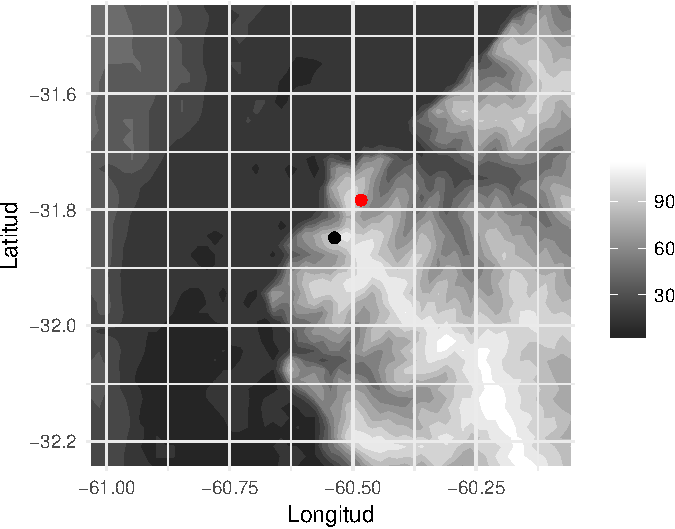
\includegraphics{Tesis_files/figure-latex/topografia-1} 

}

\caption[Topografía de la región en estudio en metros sobre el nivel del mar.]{Topografía de la región en estudio en metros sobre el nivel del mar. El punto negro indica la ubicación del Radar INTA Paraná, el punto rojo indica la ubicación de la estación Paraná Aero. Datos ETOPO1 1 Arc-Minute Global Relief Model NOAA (Amante y Eakins, 2009). \label{topografia}}\label{fig:topografia}
\end{figure}

La elevación de la región elegida muestra un mínimo de 5 metros sobre el
nivel del mar en el lecho del río Paraná y un máximo de aproximadamente
110 metros sobre el nivel del mar sobre el margen sudeste de río donde
ubica tanto la estación meteorológica como el radar (Figura
\ref{topografia}). La región está dominada por la presencia del río y
las regiones costeras donde predominan los campos de pastizales o pasto
con excepción la ciudad de Paraná (al norte), la ciudad de Santa Fé (al
noreste) y pequeños conglomerados de casas.

\subsection{\texorpdfstring{Criterios utilizados para la selección de
los casos de estudio
\label{sec-criterios}}{Criterios utilizados para la selección de los casos de estudio }}\label{criterios-utilizados-para-la-seleccion-de-los-casos-de-estudio}

Se determinaron distintos criterios para poder identificar casos de
estudio donde se observe el desarrollo de la CLP en condiciones normales
\textbf{Cita}.

Al mismo tiempo se buscaron situaciones donde los datos de radar son
confiables. Los criterios seleccionados son los siguientes:

\begin{itemize}
\tightlist
\item
  \textbf{Viento moderado.} En estas situaciones los datos de radar son
  más confiables y permiten el desarrollo de la capa límite estable
  nocturna (Gassmann y Mazzea, 2001). Se determinó como umbral máximo 7
  m/s que corresponde a la categoría de brisa moderada en la escala de
  Beaufort.
\item
  \textbf{Cielos despejados.} Para garantizar el calentamiento desde la
  superficie y el desarrollo de una capa límite mezclada. En los casos
  donde hubo nubosidad presente, se analizó el tipo de nubosidad, el
  porcentaje de cobertura del cielo y el impacto que tuvo en la
  temperatura. Los días donde la nubosidad afectó la variación normal de
  la temperatura (descenso continuo por la noche y ascenso durante el
  día) fueron descartados.
\item
  \textbf{Verano.} Donde el calentamiento es más intenso.
\end{itemize}

Las características previas se buscaron a partir del análisis de los
datos de la estación meteorológica de superficie Paraná Aero provistos
por el SMN y de reflectividad (dBZ) del radar de Paraná para el mes de
enero de 2016.

En el primer tipo de datos se analizó la velocidad de viento, la
cobertura nubosa y la precipitación observada a cada hora. En el caso de
los datos de radar se observó la presencia de ecos meteorológicos en las
inmediaciones del radar (a una distancia menor a 150 km) en cada tiempo
disponible (aproximadamente cada 10 minutos). Un caso de estudio posible
será aquel que cumpla con las características mencionadas durante las 24
horas del día aunque es deseable que las condiciones se mantengan
durante las 12 horas previas al día en estudio ya que las
características de la capa estable nocturna puede ser influenciada por
las características de la capa mezclada del día anterior.

\section{Descripción de los datos de
radar}\label{descripcion-de-los-datos-de-radar}

El radar ubicado en Paraná (Provincia de Entre Ríos) es de doble
polarización y emite energía electromagnética en la banda C (4 a 8 GHz).
La estrategia de escaneo de la atmósfera está programada para que la
antena dé giros en sentido horizontal de 360º y cambie de elevación
sucesivamente 12 veces. El ángulo vertical varía entre 0.5° y 15.1°. El
rango del radar (distancia a la que llega la señal desde la ubicación
del radar) puede ser de 120, 240 y 480 km con una resolución espacial en
la dirección del rango de 500 m de acuerdo a la estrategia de escaneo
(Saibene et~al., 2014).

El escaneo completo del volumen de atmósfera que rodea al radar se
realiza cada 5 minutos en el rango de 120 km y de 240 km de manera
intercalada, dando como resultado 144 volúmenes de datos diarios para
cada estrategia de escaneo. Las variables disponibles en cada tiempo
incluyen la reflectividad (dBZ) y velocidad radial (\(V_r\)).

Los datos de reflectividad permitieron evaluar la presencia de nubosidad
en cada momento mientras que la velocidad radial se utilizó para
calcular el perfil de viento. La velocidad radial medida por el radar
corresponde a la velocidad de un objetivo u obstáculo en el camino del
haz. En situaciones de aire claro (sin nubosidad) es posible tener una
medida del campo de viento dentro de la capa límite usando insectos como
obstáculos.

En este trabajo se usaron datos de radar provistos por el Servicio
Meteorológico Nacional correspondientes a la estrategia de 240 km y 12
ángulos de elevación para los periodos comprendidos por cada caso de
estudio. Los datos correspondientes a la estrategia de 120 km no fueron
utilizados debido a la cantidad de ángulo de elevación disponibles fue
distinta para cada día y en todos los casos menor a 12.

Cada volumen de dato correspondiente a un tiempo de escaneo completo fue
convertido al formato CfRadial con el paquete Radx C++ (Dixon, 2010 NCAR
- National Center for Atmospheric Research) para el posterior
procesamiento y análisis. En particular se utilizó la variable de
reflectividad sin procesamiento para determinar la presencia o no de
ecos meteorológicos en el dominio cercano al radar y la velocidad radial
para la obtención de los perfiles de viento.

\section{Tratamiento de aliasing}\label{tratamiento-de-aliasing}

Un problema importante al momento de utilizar los datos de velocidad
radial es la contaminación por aliasing ya que afecta significativamente
la calidad de los perfiles de viento finales, de acuerdo a Gao y
Droegemeier (2004) un 3\% de contaminación por aliasing puede generar un
error cuadrático medio del 50\% en el perfil de viento medio a partir de
la técnica VAD. El aliasing es la superposición de la señal de radar y
ocurre cuando la velocidad real supera a la velocidad de Nyquist
(\(V_N\)). Este parámetro es intrínseco a las características del radar
ya que depende de la frecuencia y estrategia de escaneo y en particular
de la frecuencia de repetición del pulso o señal que emite.

En el caso del radar de Paraná con la estrategia de escaneo de 240km de
rango, tiene una \(V_N = 6.7 m/s\) por lo que cualquier velocidad mayor
se verá afectada por el aliasing. Esto puede verse en la Figura
\ref{aliasing}, las regiones con aliasing son aquellas que donde el
valor de la velocidad radial salta al extremo opuesto de la escala.

Existen muchos algoritmos que buscan solucionar el problema del aliasing
(por ejemplo Haase y Landelius, 2004; Lim y Sun, 2010) con distinto
grado de éxito. Una opción válida es el algoritmo de corrección de
aliasing basado en regiones similares disponible en la librería PyART
(Helmus y Collis, 2016) disponible en Collis (2016). Este algoritmo
busca regiones con velocidad radial similar y transforma el rango de la
variable hasta que todas las regiones fueron corregidas de tal manera de
obtener un campo continuo. El campo de velocidad radial sin aliasing
obtenido utilizando este algoritmo se muestra en la Figura
\ref{no-aliasing}.

A partir de la exploración visual puede observarse que el algoritmo
resuelve el problema de manera satisfactoria en mayor parte del dominio.
Sin embargo se observa una zona en el borde inferior donde la mágnitud
de la variable es anómalamente alta. Algunas discontinuidades se
observaron también en otros casos. Se decidió utilizar este algoritmo
para preprocesar todos los volúmenes de datos de radar y se incorporaron
algunos controles de calidad al algoritmo de VAD desarrollado (Ver
Sección \ref{sec-vad}).

\begin{figure}
\subfloat[Con aliasing \label{aliasing}\label{fig:aliasing1}]{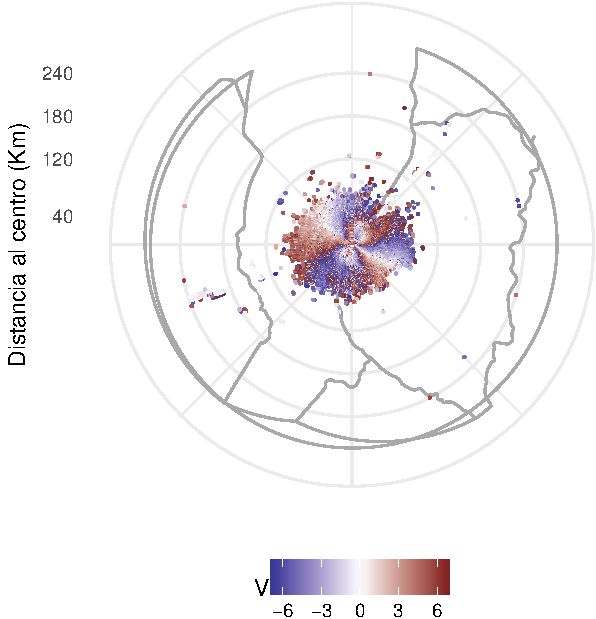
\includegraphics[ ]{Tesis_files/figure-latex/aliasing-1} }\subfloat[Sin aliasing \label{no-aliasing}\label{fig:aliasing2}]{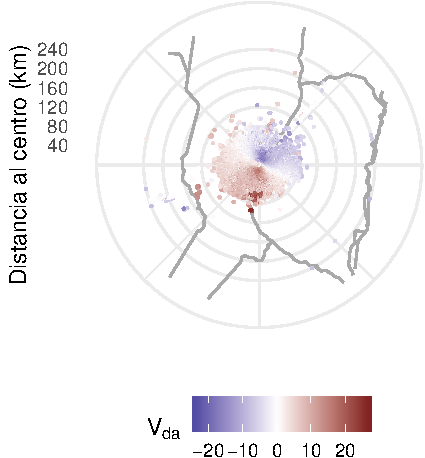
\includegraphics[ ]{Tesis_files/figure-latex/aliasing-2} }\caption{Velocidad radial (m/s) observada a las 06 UTC por el radar de Paraná en la elevación $1.3^{\circ}$ y $V_N = 6.7 m/s$. Notar las escalas diferentes.}\label{fig:aliasing}
\end{figure}

\section{\texorpdfstring{Visualización Azimutal de la Velocidad
\label{sec-vad}}{Visualización Azimutal de la Velocidad }}\label{visualizacion-azimutal-de-la-velocidad}

A medida que el radar rota en la dirección azimutal, mide la velocidad
de los objetivos para cada ángulo y rango de manera continua y en
función del azimut. A esto se le da el nombre de Visualización Azimutal
de la Velocidad o por sus siglas en inglés VAD (por Velocity Azimuth
Display, Lhermitte (1962)) y se muestra en la Figura \ref{vad}. Si el
campo de viento es horizontalmente homogéneo, la velocidad radial media
tiene un comportamiento sinusoidal en función del azimut.

\begin{figure}

{\centering 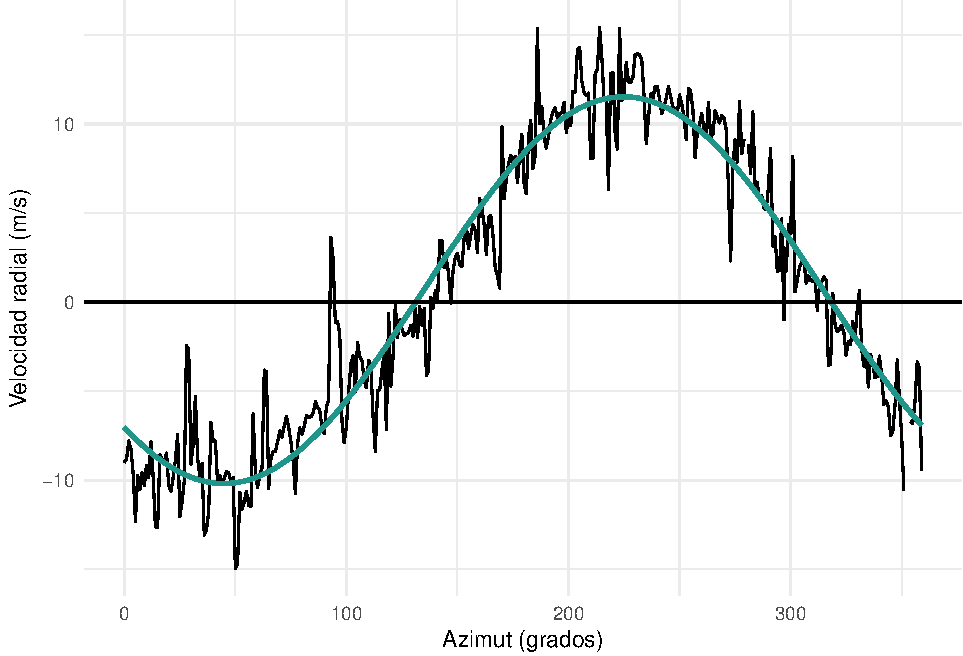
\includegraphics{Tesis_files/figure-latex/vad-1} 

}

\caption{Velocidad radial (m/s) en función del azimut (grados) para un rango y ańgulo de elevación fijos. En color se  ajusta una función sinusoidal a los datos. \label{vad}}\label{fig:vad}
\end{figure}

Esta variable corresponde es la componente radial del viento, es decir,
la proyección del viento en la dirección de la propagación del haz de
radar. Los valores negativos corresponden a movimiento hacia el radar y
valores positivos movimientos desde el radar, mientras que el valor nulo
ocurre en las regiones donde el viento es perpendicular a la trayectoria
del haz y por lo tanto su proyección es cero.

En días de buen tiempo y aire claro la señal que recibe el radar
corresponden a los insectos que se encuentran en la capa límite.
Diferentes autores han analizado la validez de la estimación del viento
a partir de estos blancos. Si bien en algunos casos los insectos pueden
ser considerados blancos pasivos, en otros casos, dependiendo del tamaño
y características del insecto, pueden moverse con velocidad y dirección
propias (Rennie, 2014). De acuerdo a Hannesen et~al. (2014), una posible
solución a este problema podría ser el uso de variables polarimétricas
que permitan determinar la orientación y dirección de desplazamietno de
los insectos para luego corregir la variable \(V_r\) observada. En este
trabajo si bien no se analizó la calidad de los datos desde este punto
de vista individualmente, si se tuvieron en cuenta controles de calidad
para disminutir errores.

Usando el concepto de la Visualización Azimutal de la Velocidad
distintos autores han desarrollado técnicas para obtener el perfil
vertical de viento real a partir del viento radial o su gradiente con
diferentes grados de complejidad. Estas técnicas son también son
llamadas VAD (o sus derivaciones). Algunos de estos algoritmos permiten
estimar variaciones del viento dentro del dominio siempre que éstas sean
lineales. Browning y Wexler (1968), unos de los primeros autores en
aplicar este concepto, desarolló una técnica utilizando series de
Fourier para obtener variables del campo del viento descompuesto en la
parte divergente, la parte rotacional y la componente de deformación
válida para casos donde el campo de viento es horizontalmente homogeneo.

Una variación del VAD, el EVAD (por las siglas en inglés de
Visualización Azimutal de la Vecidad Extendida) fue desarollado por
Matejka y Srivastava (1991). En esta técnica se incorpora el uso de
pesos al estimar las variables para tener en cuenta los errores en los
datos originales y el análisis de los residuos obtenidos a partir de las
regreciones calculadas. De acuerdo a los autores, esto permite el uso
del algoritmo en situaciones donde la cortante vertical del viento es
fuerte, ihnomogeneidades en el campo horizontal o insuficientes datos de
radar. Posteriormente Gao et~al. (2004) desarolló el GVAD (por las
siglas en inglés de Visualización Azimutal del Gradiente de la Vecidad)
que permite obtener el perfil vertical del viento aún en casos donde los
datos están contaminados por aliasing utilizando el gradiente del la
velocidad radial. Si bien esta técnica es una mejora sustancial, es muy
sensible a errores aleatorios y sistemáticos causados por el aliasing.
Xu et~al. (2010) también busca soluciar el problema de la contaminación
por aliasing utilizando un algoritmo que ajusta los datos con aliasing a
un modelo de viento uniforme. Posteriormente el mismo autor modifica
este algoritmo a partir de un un método variacional que permite eliminar
la condición de homogeneidad del campo de viento.

Para esta tesis se desarrolló un algoritmo para el cálculo del VAD
siguiendo a Browning y Wexler (1968) debido a la simpleza de la técnica
pero además se incluyeron controles de calidad específicos para asegurar
la validez de los resultados, algunos de los cuales también fueron
implementados por los autores mencionados.

\subsection{Desarrollo matemático}\label{desarrollo-matematico}

El viento radial medido por el radar para un ángulo de elevación
\(\theta\) y rango \(r\) determinado puede expresarse en función del
azimut \(\phi\):

\begin{equation}
\label{eq-vr1}
V_r =  v \cos(\theta) \cos(\phi) + u \cos(\theta) \sin(\phi) - w \sin(\theta)
\end{equation}

Donde \(u\), \(v\) y \(w\) son las componentes del viento en coordenadas
cartesianas.

La Ecuación \ref{eq-vr1} puede ser expresada como suma de una serie de
Fourier de la forma:

\begin{equation}
\label{eq-vr2}
V_r =  \frac{1}{2}a_0 + \sum_{n = 1}^{\infty} (a_n \cos(n\phi) + b_n \sin(n \phi)) 
\end{equation}

Para \(n=1\), los coeficientes de Fourier están asociados al viento en
el centro del dominio de escaneo (con subíndice 0) como:

\begin{equation} \label{eq-vr3}
\begin{aligned}
a_0 = r \cos(\theta)\left ( \frac{\overline{\partial u}}{\partial x} + \frac{\overline{\partial v}}{\partial y} \right) + 2 w \sin(\theta) \\
a_1 = u_0 \cos(\theta) \\
b_1 = v_0 \cos(\theta) \\
a_2 = \frac{1}{2} r \cos(\theta)\left ( \frac{\overline{\partial u}}{\partial x} - \frac{\overline{\partial v}}{\partial y} \right) \\
b_2 = \frac{1}{2} r \cos(\theta)\left ( \frac{\overline{\partial u}}{\partial y} + \frac{\overline{\partial v}}{\partial x} \right)
\end{aligned}
\end{equation}

A partir de esto es posible ajustar cada anillo de datos de radar, es
decir los datos para cada \(\theta\) y \(r\) realizando una regresión
lineal de la forma:

\begin{equation}
\label{eq-vr4}
V_r \sim a_1\cos \phi + b_1 \sin \phi
\end{equation}

Los coeficientes \(a_0\), \(a_2\) y \(b_2\) dan información sobre la
divergencia horizontal y otras características de la variación viento.
Estos no fueron estimados por el algoritmo pero es posible su
implementación en futuros trabajos.

Finalmente la velocidad y dirección del viento pueden ser calculadas a
partir de los coeficientes (Ecuaciones \ref{eq-vr3}).

Velocidad:

\begin{equation}
\label{eq-vr5}
V = \frac{(a_{1}^{2} + b_{1}^{2})^{1/2}}{\cos(\theta)}
\end{equation}

Dirección:

\begin{equation}\label{eq-vr6}
\alpha = \frac{\pi}{2}-\tan^{-1}(\frac{a_1}{b_1}) \; \; si \; b_1 < 0 
\end{equation}\begin{equation}\label{eq-vr7}
\alpha = \frac{3\pi}{2}-\tan^{-1}(\frac{a_1}{b_1}) \; \; si \; b_1 > 0
\end{equation}

El resultado de lo anterior da un valor de la magnitud del viento y su
dirección para cada anillo asociado a un ángulo de elevación y rango
determinado. Para calcular la altura de cada anillo es necesario conocer
la propagación del haz del radar. Ésta depende del indice de refracción
de la atmósfera (N) y este a su vez de la densidad del aire y por lo
tanto de las condiciones de temperatura y humedad del momento. Existen
distintas metodologías para calcular la propagación del haz del radar
(Zeng et~al., 2014) que varían en complejidad y precisión.

En el algoritmo de VAD desarrollado se aplica el modelo 4/3 del radio de
la Tierra. Este modelo es utilizado por la mayoría de los programas de
procesamiento de datos de radar ya que pese a su simpleza (no toma en
cuenta las condiciones de la atmósfera) es aceptable para cualquier
ángulo de elevación usado, alturas máximas de entre 10 y 20 km siempre
que el gradiente de N esté alrededor de \(-1/a\) donde \(a\) es el radio
de la Tierra (Doviak y Zrnić, 1993).

Por otro lado se calcula la raíz del error cuadrático medio asociado a
cada anillo (\(rmse_a\)) para estimar la diferencia entre las
observaciones y el modelo estimado:

\begin{equation}\label{eq-vr8}
rmse_a = \sqrt {\sum \frac {(V_r - V_{rmod} )^2} {n-3}}
\end{equation}

donde \(n\) es el número de observaciones presentes en un anillo
particular.

\begin{figure}

{\centering 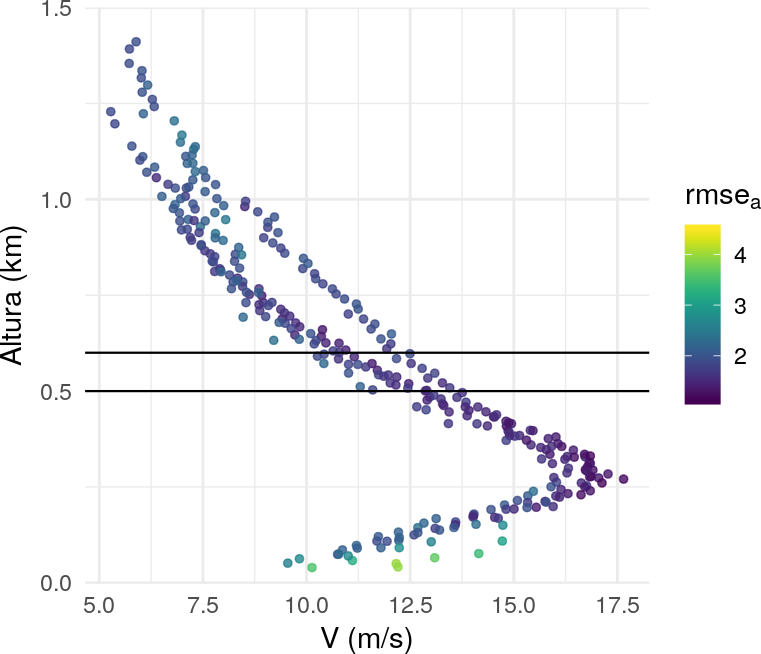
\includegraphics{Tesis_files/figure-latex/evad-1} 

}

\caption{Velocidad del viento (m/s) en función de la altura para los distintos ángulos de elevación (puntos) y perfil final obtenido luego del primedio pesado (linea) calculados con VAD. \label{evad}}\label{fig:evad}
\end{figure}

En la Figura \ref{perfil-rmse} se muestra el valor de la magnitud del
viento calculado a partir de cad anillo válido y en color el valor de
\(rmse_a\) asociado para un caso de ejemplo. La dispersión de los datos
varía con la altura pero se mantiene la forma del perfil con un
\(rmse_a\) medio de 2.01 m/s.

Para obtener el perfil vertical de viento que se observa en la Figura
\ref{perfil-rmse} se calcula un promedio pesado de los datos de anillos
individuales correspondientes a cada capa de atmósfera para obtener un
valor para cada punto de una grilla vertical equiespaciada
preestablecida.

El algoritmo identifica los datos de \(V\) para cualquier rango y ángulo
de elevación que se encuentran en \(z \pm d/2\) donde \(z\) es el punto
de grilla y \(d\) es la resolución espacial de la grilla vertical. Para
obtener el valor promedio de \(V\) correspondiente a la altura \(z\)
calcula un promedio pesando la variable por el \(rmse_a\) y la distancia
de cada anillo al radar \(r\). De esta manera los anillos con mayor
error y más alejados a punto donde se está estimando la velocidad y
dirección del viento tienen menor influencia en el resultado final. Si
bien el \(rmse_a\) y \(r\) tienen magnitud distinta se observó que el
primero tiene mayor influencia en el promedio pesado y que el \(r\)
permite una mayor coherencia de los datos.

\begin{equation}\label{eq-vr9}
\bar{V} = \frac {\sum w_i V_i} {\sum w_i}
\end{equation}

Donde \(w_i = \frac {1}{rmse_{ai} + r_i}\) y el subíndice \(i\) cuenta
la cantidad de datos para cada intervalo \(z \pm d/2\). De manera
análoga se calcula las componentes \(u\) y \(v\) y a partir de estas, la
dirección del viento para cada punto de grilla vertical. Este cálculo no
se realiza con la dirección del viento estimada con las Ecuaciones
\ref{eq-vr6} y \ref{eq-vr7} porque al ser una variable cíclica, el
promedio puede generar errores.

Finalmente se calcula el error de estimación asociado a cada punto de
dos maneras:

\begin{itemize}
\tightlist
\item
  \textbf{\(rmse_1\)}
\end{itemize}

\begin{equation}\label{eq-vr10} 
rmse_1 = \frac{\sigma}{\sqrt{n}}
\end{equation}

Donde \(n\) es la cantidad de anillos en esa capa y
\(\sigma^{2}= \frac{\sum (V_i - \bar{V})^2 /rmse_{ai}^2}{\sum 1/rmse_{ai}^2}\)
con \(\bar{V}\) el promedio pesado de la velocidad del viento para la
capa.

Este error relativo da cuenta de la distancia entre la velocidad
promedio calculada para ese nivel y el valor de cada anillo pesada por
el error del anillo. De esta manera si el \(rmse_{ai}\) es grande la
diferencia \((V_i - \bar{V})^2\) tiene menor peso en el error del nivel.
Es importante notar que \(V_i\) y \(\bar{V}\) no están necesariamente a
la misma altura ya que \(\bar{V}\) es el promedio de muchos \(V_i\)
dentro de una capa.

\begin{itemize}
\tightlist
\item
  \textbf{\(rmse_2\)}
\end{itemize}

\begin{equation}\label{eq-vr11}
rmse_2 = \sqrt{\frac{1}{\sum \frac{1}{rmse_{ai}^2}}}
\end{equation}

Este rmse no toma en cuenta la posible dispersión de los valores
individuales de los anillos respecto del valor medio pero retiene el
error cuadrático medio de cada anillo y calcula la raíz del error
cuadrático medio del nivel como la suma de la inversa de los errores
individuales.

\subsection{Controles de calidad de los
datos}\label{controles-de-calidad-de-los-datos}

El algoritmo de VAD desarrollado incluye algunos controles de calidad
para evitar errores asociados a problemas intrínsecos a los datos de
radar.

\subsubsection{Antes del ajuste de los
datos}\label{antes-del-ajuste-de-los-datos}

Permiten determinar cuales son los anillos de datos válidos y eliminar
posibles errores aleatorios.

\begin{itemize}
\tightlist
\item
  \textbf{Ángulos de elevación seleccionados:} La presencia de ecos de
  terreno pueden generar que los campos de velocidad radial para los
  primeros ángulos de elevación sean muy ruidosos y sin coherencia
  espacial. En el otro extremo, en caso de ser necesario,se puede
  eliminar los ángulos superiores. Por lo tanto es posible seleccionar
  el rango de ángulos a ser analizados y utilizados en el cálculo del
  VAD con el \emph{Ángulo mínimo} y el \emph{Ángulo máximo}.
\item
  \textbf{Selección del dominio de cálculo:} Otro posibilidad para
  evitar los ecos de terreno es definir un \emph{Radio interior} por
  debajo del cual no se incluyen los datos para el cálculo de VAD. En el
  otro extremo, es posible definir un \emph{Radio exterior} para limitar
  el uso de datos muy lejanos al centro del volumen de escaneo. Esto es
  importante para evitar inhomogeneidades en el campo de viento
  horizontal.
\item
  \textbf{Cantidad de datos por anillo:} el algoritmo cuenta la cantidad
  de datos válidos por anillo y se define un porcentaje de datos
  faltantes (NaN) límite respecto del total para descartar el anillo,
  por ejemplo 20\%. Si se excede al máximo definido o \emph{NaN máximo}
  el anillo es descartado. De esta manera se evita la utilización de
  anillos donde la señal es muy débil.
\item
  \textbf{Hueco continuo en un anillo:} Además de los datos faltantes
  ubicados de manera aleatoria a lo largo de un anillo, los huecos
  continuos pueden ocurrir debido a la falta de señal en una determinada
  región. De acuerdo a Matejka y Srivastava (1991) esto puede generar
  importantes errores en el resultado final, por lo tanto cuando el
  hueco o \emph{Gap máximo} es mayor a 30° de azimut, el anillo se
  descarta.
\item
  \textbf{Errores aleatorios:} Los errores aleatorios producto de ruido
  del instrumento pueden ser eliminados utilizando un filtro pasa bajo
  (Gao y Droegemeier, 2004). Este control no elimina anillos pero
  produce un suavizado de los datos de cada anillo de manera
  independiente. Es necesario definir la cantidad de datos o \(Pesos\)
  que se utilizaran para calcular el filtro en cada punto.
\end{itemize}

\subsubsection{Luego del ajuste de los
datos}\label{luego-del-ajuste-de-los-datos}

\begin{itemize}
\tightlist
\item
  \textbf{R cuadrado:} El \(r^2\) del modelo ajustado (Ecuación
  \ref{eq-vr4}) permite obtener una medida de de la calidad de ese
  modelo respecto de las observaciones. A partir de la exploración de
  resultados preliminares se observó que la definición de un umbral
  mínimo para el \(r^2\) permite descartar anillos que pese a no tener
  datos faltantes eran erróneos.
\end{itemize}

\subsection{Validación del algoritmo}\label{validacion-del-algoritmo}

Una manera posible de validar los resultados del VAD es comparando
cualitativa o cuantitativamente el perfil vertical de viento generado
con los datos de un radiosondeo en el mismo momento. Debido a la
inexistencia de sondeos en la región de Paraná se exploró la posibilidad
de utilizar datos del Radar INTA Anguil que se encuentra en la provincia
de La Pampa y radiosondeos de la estación del SMN Santa Rosa Aero. Si
bien el radar y la estación meteorológica no están en la misma
ubicación, se encuentran a unos 30 km de distancia y por lo tanto la
estación está dentro del dominio de escaneo del radar (Figura
\ref{topo-anguil}). Sin embargo se encontró que la señal de \(V_r\) en
días de cielo claro es muy pobre y por lo tanto al realizar
losccontroles de calidad impuestos en el algoritmo, el perfil de viento
final no llega a los 1000 m.

\begin{figure}

{\centering \includegraphics{Tesis_files/figure-latex/topo-anguil-1} 

}

\caption{Topografía de la región del radar Anguil en metros sobre el nivel del mar. El punto negro indica la ubicación del Radar INTA Anguil, el punto rojo indica la ubicación de la estación Santa Rosa Aero. Datos ETOPO1 1 Arc-Minute Global Relief Model NOAA (Amante y Eakins, 2009). \label{topografia}}\label{fig:topo-anguil}
\end{figure}

Pero también es posible reconstruir un campo de velocidad radial
sintética interpolando la velocidad medida por la radiosonda a la grilla
del radar utilizando la Ecuación \ref{eq-vr1}. En este proceso se asume
que el campo de viento tridimensional varía linealmente. Este campo de
velocidad radial sintética \(V_{rs}\) puede ser re transformado a un
perfil vertical de viento utilizando el VAD y comparado con el sondeo
original para determinar la validez del algoritmo.

Para este segundo método de validación se utilizaron un volumen de datos
del Radar INTA Anguil del 05 de enero de 2016 a las 12 UTC y los datos
del radiosondeo de la estación del SMN Santa Rosa Aero para la misma
hora. Además, dado que el resultado de la interpolación del viento real
da un campo homogéneo, sin errores o datos faltantes, se aplicaron
distintas fuentes de errores para que la validación sea más realista.

\subsubsection{Pruebas de validación para distintos errores y datos
faltantes}\label{pruebas-de-validacion-para-distintos-errores-y-datos-faltantes}

\begin{itemize}
\tightlist
\item
  \textbf{Sin datos faltantes ni errores (SE)}
\end{itemize}

Se obtiene el \(V_r\) interpolado a la grilla del radar de Anguil (con
una estrategia de escaneo hasta 120 km de radio y 8 ángulos de
elevación) a partir del sondeo. Como los datos de sondeo llegan hasta
los 30 km de altura, hay información disponible para interpolar los
datos de \(V_r\) para todos los ángulos de elevación y para cualquier
rango. Sin embargo esto genera muchos más datos de los disponibles
normalmente. Es de esperar que el VAD resultante sea muy similar al
sondeo inicial pero esta primera validación también permite verificar
que la transformación de \(V\) a \(V_r\) es correcta.

\begin{figure}

{\centering \subfloat[Datos de radar \label{radar}\label{fig:validacion1}]{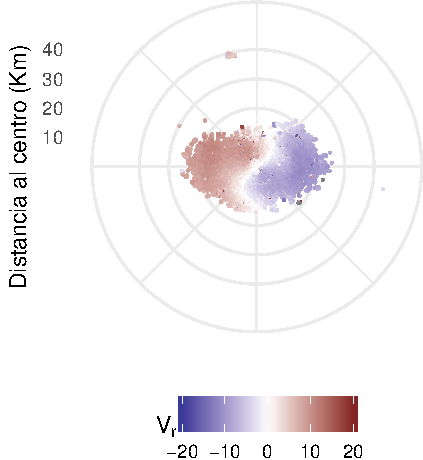
\includegraphics[ ]{Tesis_files/figure-latex/validacion-1} }\subfloat[Sin errores \label{se}\label{fig:validacion2}]{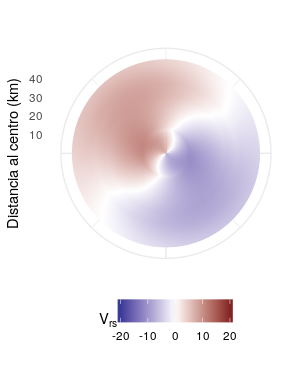
\includegraphics[ ]{Tesis_files/figure-latex/validacion-2} }\newline\subfloat[Con errores \label{ce}\label{fig:validacion3}]{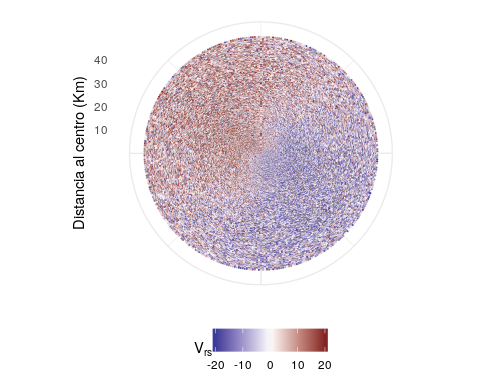
\includegraphics[ ]{Tesis_files/figure-latex/validacion-3} }\subfloat[Con errores + NAs \label{na}\label{fig:validacion4}]{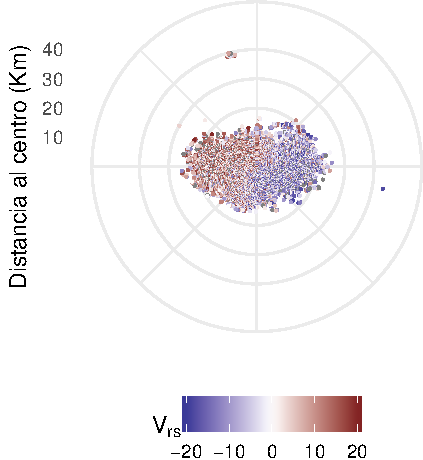
\includegraphics[ ]{Tesis_files/figure-latex/validacion-4} }

}

\caption{Velocidad radial (m/s) observada a las 12 UTC por el radar de Anguil en la elevación $1.3^{\circ}$ y la misma variable transformada a partir del sondeo de la estación Santa Rosa Aero para la misma hora \label{validacion}}\label{fig:validacion}
\end{figure}

En la Figura \ref{validacion} se puede observar el campo de \(V_r\)
observado por el radar (a) y el campo de \(V_{rs}\) obtenidos a partir
del sondeo (b). Cualitativamente se observa que tanto la magnitud como
la dirección del viento son similares pero también que el \(V_rs\) cubre
totalmente el dominio mientras que la señal del \(V_r\) se extingue a
los 15 km de rango. Cuantitativamente la diferencia \(V_r - V_{rs}\) es
grande en puntos localizados pero el error absoluto medio es de 2.08
m/s, un valor razonable teniendo en cuenta que las observaciones son
realizadas por instrumentos distintos.

\begin{itemize}
\tightlist
\item
  \textbf{Con errores aleatorios (EA)}
\end{itemize}

Para realizar una validación más realista se agregaron errores
aleatorios al campo de \(V_{rs}\), esto además permite analizar la
sensibilidad del algoritmo a este tipo de errores.

El nuevo campo perturbado será:

\begin{equation} \label{eq-vr12}
V_{rs}'  = V_{rs} + \alpha \varepsilon(0,1)
\end{equation}

Donde \(\alpha\) es la amplitud del error y \(\varepsilon\) es un número
aleatorio con distribución normal, \(\mu = 0\) y \(\sigma= 1\).

En la Figura \ref{ce} se muestra el campo resultante utilizando
\(\alpha = 1 m/s\), rápidamente se ve la variabilidad impuesta y también
la disminución en la coherencia horizontal aunque se mantiene
aproximadamente el signo de la variable en las distintas regiones.

\begin{itemize}
\tightlist
\item
  \textbf{Con errores aleatorios y datos faltantes (EA+NA)}
\end{itemize}

Otro problema importante en los datos de radar es la ausencia de señal,
esto se ve como datos faltantes (NAs). Para analizar el efecto de los
datos faltantes se aplicó una máscara de NAs al campo de \(V_{rs}'\) de
tal manera que sean los mismo NAs presentes en el volumen de datos de
radar utilizados para que la distribución de Nas sea realista (Figura
\ref{na}).

\subsubsection{Perfiles obtenidos}\label{perfiles-obtenidos}

En la Figura \ref{validacion-perfiles} se muestra el perfil del sondeo
para los primeros 3 km de altura, los perfiles calculado con VAD a
partir de los distintos campos sintéticos y en negro se nuestra el
perfil vertical obtenido a partir de las observaciones del radar para
esa hora. En cuanto a la magnitud no se ven diferencias importantes
entre el sondeo y los perfiles sintéticos. Al observar el detalle de los
primeros 1000 metros de altura, la diferencia es menor a 0.5 m/s en
todos los casos. Tampoco se observó sensibilidad al aumento de la
amplitud de error (no se muestra).

\begin{figure}
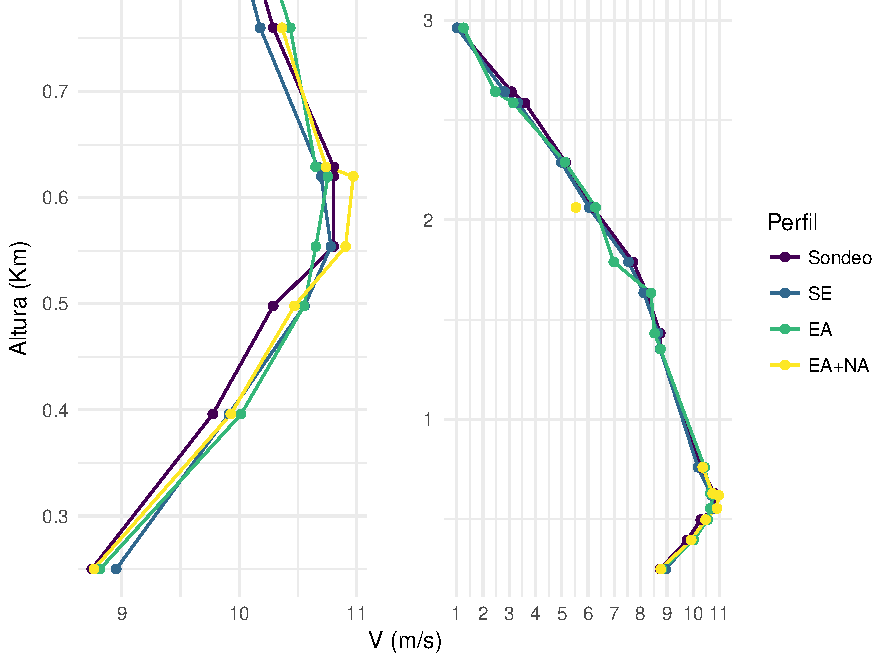
\includegraphics[ ]{Tesis_files/figure-latex/validacion-perfiles-1} \caption{Viento medio (m/s) en función de la altura a partir del sondeo, y las distintas pruebas de validación a la izquierda y el detalle ampliado del máximo en niveles bajos \label{validacion-perfiles}}\label{fig:validacion-perfiles}
\end{figure}

\begin{longtable}[]{@{}lrr@{}}
\caption{Errores calculados para las distintas pruebas de validación.
\label{validacion-errores}}\tabularnewline
\toprule
Prueba & rms & rre\tabularnewline
\midrule
\endfirsthead
\toprule
Prueba & rms & rre\tabularnewline
\midrule
\endhead
SE & 0.1613 & 0.0194\tabularnewline
EA & 0.3020 & 0.0364\tabularnewline
EA+NA & 0.1778 & 0.0214\tabularnewline
\bottomrule
\end{longtable}

Esto puede verificarse con el cálculo de distintos errores (Gao y
Droegemeier, 2004): la raíz del error cuadrático medio
(\(rms = \sqrt{ \frac{\sum (V-V_{ref})^2}{N} }\)) y el error relativo al
rms (\(rre = \sqrt{ \frac{\sum (V-V_{ref})^2}{\sum (V_{ref})^2} }\))
donde \(V_{ref}\) corresponde a la variable de referencia, en este caso
el sondeo. Los resultados se muestran en la Tabla
\ref{validacion-errores} y como puede observarse no hay un aumento
importante al incorporar errores aleatorios y disminuye al quitar datos
en la prueba EA+NA ya que los errores calculados son sensibles a la
cantidad total de datos.

El efecto más importante en las pruebas de validación corresponde a la
presencia de NAs. La falta de datos en distintas regiones para rangos a
partir de 10 a 15 km impide el cálculo del perfil por encima de 800
metros (con excepción de un punto a los 2000 metros de altura).

Si se compara cualitativamente los perfiles de viento obtenidos con el
sonde y el perfil calculado con VAD a partir de los datos de radar se
observa que estos no coinciden. Además de la falta de datos por encima
de los 800 m (debido a la débil señal del radar), la magnitud del viento
observado por el radar es siempre menor y con una diferencia de hasta 2
m/s. Tampoco se observa una similitud en la forma de los perfiles pero
puede deberse, en parte, a los pocos datos disponibles.

\subsection{Configuración del algoritmo
elegida}\label{configuracion-del-algoritmo-elegida}

En la Tabla \ref{parametros} se detallan los valores utilizados en los
distintos parámetros necesarios para el algoritmo VAD que se mantuvieron
para todos los casos de estudio.

\begin{table}

\caption{\label{tab:parametros}Parámetros utilizados en el cálculo del VAD y la construcción de la grilla vertical para todos los casos. \label{parametros}}
\centering
\begin{tabular}[t]{lll}
\toprule
Algoritmo & Parámetro & Valor\\
\midrule
 & Ángulo mínimo & 1.3°\\
\cmidrule{2-3}
 & Ángulo máximo & 11.8°\\
\cmidrule{2-3}
 & Radio interior & 0.3 km\\
\cmidrule{2-3}
 & Radio exterior & 40 km\\
\cmidrule{2-3}
 & NaN máximo & 72\\
\cmidrule{2-3}
 & Gap máximo & 30\\
\cmidrule{2-3}
 & Pesos & -\\
\cmidrule{2-3}
\multirow{-8}{*}{\raggedright\arraybackslash VAD} & R cuadrado & 0.8\\
\cmidrule{1-3}
 & Altura mínima & 0.1 Km\\
\cmidrule{2-3}
 & Altura máxima & 3 Km\\
\cmidrule{2-3}
\multirow{-3}{*}{\raggedright\arraybackslash Grilla vertical} & Espaciado & 0.1 Km\\
\bottomrule
\end{tabular}
\end{table}

\section{Consistencia temporal de las
observaciones}\label{consistencia-temporal-de-las-observaciones}

Ya que uno de los objetivos de esta tesis es estudiar la evolución del
viento a lo largo del día, es importante asegurar cierta consistencia
temporal en los datos. La inconsistencia temporal puede deberse a que
cada volumen de datos no es medido de manera instantánea si no que
demora algunos minutos. Si bien en periodos sin cambios sinópticos
importantes no se espera variaciones bruscas del viento, es posible que
variaciones menores a los 10 minutos (resolución temporal de los datos
de radar) estén afectando la consistencia temporal.

Para solucionar este problema se aplicó un suavizado pesado localmente o
LOWESS (LOcally WEighted Scatterplot Smoothing, Cleveland (1979)).
LOWESS es un método de regresión no paramétrica y por lo tanto no es
necesario asumir que los datos tienen algún tipo de distribución
particular. Esto lo hace un método flexible al representar el
comportamiento de los datos. Por otro lado la estimación para cada punto
se realiza utilizando la información de datos vecinos. Para esto se
especifica cuantos datos vecinos se utilizaran para estimar cada punto
local como una fracción del total de datos.

En la Figura \ref{lowess} se muestra la variación de la velocidad del
viento con el tiempo a 500 m de altura donde se identifican dos momentos
donde la variación del viento da saltos bruscos, alrededor de las 03 y
las 08 UTC. Al aplicar el LOWESS el resultado es un suavizado de la
variable que elimina los saltos bruscos y mejora la coherencia.

\begin{figure}

{\centering \includegraphics{Tesis_files/figure-latex/lowess-1} 

}

\caption{Velocidad del viento a lo largo del tiempo para el 14 de enero de 2016 a 500 m de altura (negro) y la misma variable luego de la aplicación del LOWESS (color). \label{lowess}}\label{fig:lowess}
\end{figure}

\textbf{Necesito mostrar como quedan los datos acá? No quiero spoilear
los resultados}

\section{Procesos asociados a la CLP}\label{procesos-asociados-a-la-clp}

El estudio de los procesos que ocurren en la CLP es un desafío cuando no
se cuenta con datos de la turbulencia. En esta tesis se abordan procesos
que pueden ser estudiados a partir de los perfiles de viento y las
variables de superficie.

\subsection{Determinación del estado de la
turbulencia}\label{determinacion-del-estado-de-la-turbulencia}

El número de Richardson puede ser utilizado como un estimador de la
estabilidad dinámica (Stull, 1988) y por lo tanto de la turbulencia
presente. Su definición surge como el cociente de los términos de
producción mecánica y térmica de la turbulencia en la ecuación de
energía cinética turbulenta de un fluido gaseoso (Stull, 1988). A partir
de suponer válida la teoría K (Pasquill y Smith, 1983) y que los
coeficientes de intercambio turbulento de calor sensible y de cantidad
de movimiento son iguales, es posible escribir el número de Richardson
en función de los gradientes verticales de viento y temperatura
potencial:

\begin{equation} \label{eq-ri1}
R_i = \frac{\frac{g}{\overline{\theta_v}} \frac{\partial \overline{\theta_v}}{\partial z}}
{\left [ \left (\frac{\partial \overline{u}}{\partial z} \right )^2 + \left (\frac{\partial \overline{v}}{\partial z} \right )^2  \right]}
\end{equation}

El signo de este número permite clasificar la evolución de la
turbulencia en dos clases: estables (\(R_i\) \textgreater{} 0) e
inestables (\(R_i\) \textless{} 0). EEl numerador de la Ecuación da
cuenta de la disponibilidad de energía asociada a procesos de empuje
térmico que favorecen la destrucción o inhiben la turbulencia en
condiciones estables y la producen en condiciones inestables. El
denominador corresponde a la producción mecánica o por cortante. De
acuerdo a Stull (1988) la turbulencia puede mantenerse si \(R_i\) es
menor a un valor umbral (\(R_T\)), ya que por encima de este umbral (en
general \(R_T = 1\)), la inhibición de la turbulencia se incrementa
tendiendo a estabilizar el estado del flujo y volverlo laminar.

Debido a que la estimación de los gradientes suele ser difícil, estos
tienden a ser expresados en términos de observaciones discretas. Surge
así el número de Richardson Bulk:

\begin{equation} \label{eq-ri2}
R_b = \frac{g \, \Delta \overline{\theta_v} \, \Delta z}{\overline{\theta_v} \, [(\Delta \overline{u}^2) + [(\Delta \overline{v}^2)]}
\end{equation}

Para obtener el \(R_b\) en cada tiempo y su variación con la altura es
necesariocontar con el perfil vertical de temperatura virtual
(\(\theta_v\)) y de la velocidad del viento. Debido a que solo se cuenta
con el valor de la temperatura en superficie, se utilizó la siguiente
aproximación válida para estimar el número de Richardson en el periodo
estable:

\begin{equation} \label{eq-ri3}
R_i \sim \frac{(g  \: (\theta_i - \theta_f)/z_{máx})}{(\overline{\theta} \: (u_{máx}/z_{máx})^2)}
\end{equation}

Donde \(\theta_i\) corresponde al valor de la temperatura virtual en
superficie en el momento de transición entre la capa mezclada y el
comienzo de la capa estable nocturna, por lo tanto será la temperatura
en el tope de la capa estable asumiendo que la capa residual no se
modifica. El valor de \(\theta_f\) será la temperatura en superficie
observado. Por último \(u_{máx}\) es el valor máximo de viento observado
y \(z_{máx}\), la altura a la que ocurre este máximo y que se
considerará en este trabajo como una aproximación de la altura del tope
de la capa estable (Ver Sección \ref{sec-pbh}).

\subsection{\texorpdfstring{Altura de la capa límite
\label{sec-pbh}}{Altura de la capa límite }}\label{altura-de-la-capa-limite}

La altura de la capa límite se define como la altura a la cual las
características de la superficie no afecta la atmósfera. Las
estimaciones de esta variable son muy diversas en la literatura y
también sus aplicaciones a los modelos numéricos.

Por ejemplo la altura de la capa estable nocturna puede definirse como
la altura a la cual la intensidad de la turbulencia es una fracción del
valor en superficie mientras que la altura de la capa mezclada puede
determinarse como la altura a la que se observa el menor transporte
vertical de calor sensible.

Teniendo en cuenta los datos disponibles se determinó la altura de la
capa estable nocturna como la altura a la que ocurre el máximo de
viento.

Otro enfoque posible es el uso de la reflectividad. Por ejemplo Kaufmann
y White (1997) buscó determinar la altura a la que ocurre la inversión
térmica en invierno utilizando radares y otros instrumentos asociados
utilizando la variable SNR (Signal to Noise Ratio o relación entre la
Señal y el Ruido de la refelctividad). Por otro lado Chandra et~al.
(2010) utiliza la variación de la reflectividad con la altura observada
con un perfilador radar de viento en casos de aire claro y cielo nuboso.
Esta técnica se basa en el concepto de que en el tope de la capa límite
se observan importantes gradientes de temperatura y humedad y estos
generan un máximo local en la reflectividad. En este trabajo se exploró
de manera preliminar la posibilidad de determinar la altura de la capa
límite a partir de las variación es de la reflectividad observada por el
radar con la altura.

\textbf{Ver si resulta lo de usar dBZ o si se puede hacer algo con la
altura de la capa mezclada}

\subsection{Descripción del LLJ}\label{descripcion-del-llj}

El Jet nocturno de capas bajas o LLJ (Low Level Jet) es un fenómeno de
mesoescala caracterizado por por una corriente fuerte de viento con
máximos de entre 10 y 20 m/s que se localiza en los primeros cientos de
metros de altura (Stull, 1988). Su extensión vertical es poca pero
horizontalmente puede extenderse por cientos de kilómetros.

Existen distintos criterios para identificar el LLJ. En algunos casos se
determina un umbral mínimo para la velocidad del viento a partir del
cual se considera la existencia del LLJ siempre que este ocurra por
debajo de algún nivel o altura determinada. En otros casos, se busca que
el viento sea supergeostrófico. En este trabajo se utilizará el criterio
de Bonner (1968) que identifica el LLJ cuando el máximo del viento es
superior a 12 m/s y decrece al menos 6 m/s hasta el próximo mínimo o
hasta el nivel de 3 km.

El LLJ puede producirse por distintos mecanismos entre los que se pueden
nombrar la topografía, baroclinicidad asociada a pendientes del terreno,
frentes y oscilaciones inerciales. En algunas situaciones, varios
mecanismos pueden contribuir a la formación del LLJ de manera conjunta y
estos son los que determinan las características del fenómeno.

En este trabajo el análisis se centra en el LLJ generado por la
oscilación inercial. De acuerdo a Blackadar (1957) luego del atardecer,
cuando no hay producción de turbulencia de origen térmico se produce un
desacople de la capa mezclada y el viento tiende a acelerarse ante la
ausencia de la fricción hacia el equilibrio geostrófico. Sin embargo la
fuerza de Coriolis genera una oscilación inercial del viento alrededor
del viento geostrófico produciendo un LLJ supergeostrófico durante el
periodo estable.

Esta oscilación puede verse en la rotación del vector del viento a lo
largo del tiempo. Para el hemisferio sur esta rotación será en sentido
antihorario. El periodo de la oscilación inercial es de \(P = 2\pi/f\),
con \(f\) el parámetro de Coriolis. A la latitud de Paraná \(P = 17.79\)
horas y por lo tanto se espera que el máximo viento ocurra para cuando
se alcanza la mitad del periodo desde el atardecer (Kallistratova y
Kouznetsov, 2012).

\section{Modelo WRF}\label{modelo-wrf}

En este trabajo se utilizó el modelo WRF versión 3.9.1 para la
realización de simulaciones numéricas que permitan comparar algunas de
las parametrizaciones de CLP disponibles: YSU (Yonsei University
Scheme), MYJ(Mellor--Yamada--Janjic) y ACM2 (Asymmetric Convection Model
2).

Las simulaciones se integraron en un dominio 1 anidado con un dominio 2
en dos direcciones. El dominio 1 se configuró con una resolución de 12 x
12 km y 105 x 105 puntos de grilla y dominio 2 con una resolución de 4 x
4 km y 253 x 253 puntos de grilla, ambos centrados en la ubicación del
radar de Paraná. Como se puede ver en la Figura \ref{dom-modelo} el
dominio abarca todo el centro y norte del país. Se utilizaron datos
geográficos con 10 minutos de resolución para el dominio superior y 2
minutos para el dominio inferior.

Ambos dominios tienen una grilla vertical de 42 niveles expresados en
coordenadas sigma-p, con una distribución hipérbolo tangencial para que
los primeros 20 niveles se ubiquen en los primeros 1800 m. La presión en
el tope del modelo es de 100 hPa. De acuerdo a Shin et~al. (2012) se
determinó que el nivel inferior se ubique en 40 msns para evitar errores
en algunas variables de superficie asociadas a la CLP.

\begin{figure}

{\centering \subfloat[Dominio utilizado en el modelo con resolución de 12 km (dominio exterior) y 4 km (dominio interior. El punto representa la ubicación del radar. \label{dom-modelo}\label{fig:dominio1}]{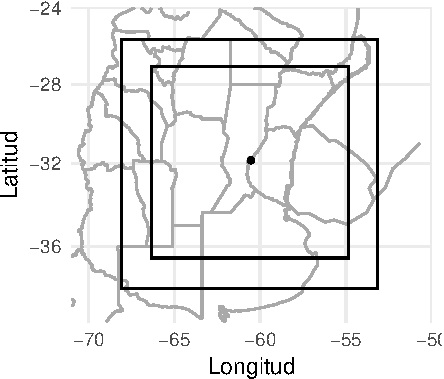
\includegraphics{Tesis_files/figure-latex/dominio-1} }\hfill\subfloat[Topografía sobre el nivel del terreno respecto de la ubicación del radar. El circulo negro corresponde al dominio de análisis, de 40km de radio y centrado en el radar. \label{dom-radar}\label{fig:dominio2}]{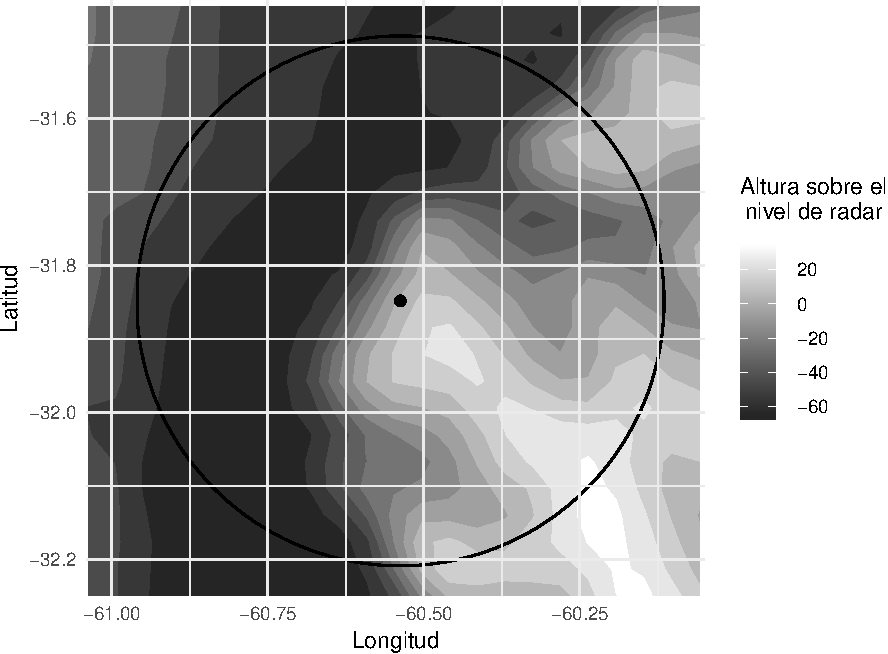
\includegraphics{Tesis_files/figure-latex/dominio-2} }

}

\caption{Dominios utilizados. \label{dominio}}\label{fig:dominio}
\end{figure}

Se realizaron simulaciones para el periodo comprendido en el Caso 1, es
decir, entre las 0600 UTC del 13 de enero a las 0000 del 15 de enero de
2016 en todos los casos. Las primeras 6 horas de simulación corresponden
al ``spin up'' del modelo y las siguientes 36 horas al período de
interés para el análisis. Si bien el estudio se centra en comparar las
observaciones del 14 de enero con las simulaciones, es importante tener
en cuenta que la capa estable nocturna puede ser muy influenciada por la
capa mezclada del día anterior, por esta razón la simulación empieza 12
horas antes.

Para las condiciones iniciales para las 0600 UTC del 13 de enero de 2016
se utilizó el Análisis Final (FNL) de National Centers for Environmental
Prediction (NCEP) con resolución de 0.25° X 0.25° y las condiciones de
borde fueron forzadas por los mismos datos cada 6 horas.

Para los procesos físicos no asociados a la CLP se usaron las siguientes
parametrizaciones: RRTMG (Rapid Radiative Transfer Model for GCMs,
Mlawer et~al. (1997)) para la radiación de onda larga, Dudhia (Dudhia,
1989) para la radiación de onda corta, WSM6 (WRF Single-Moment 6-Class
Microphysics, Hong y Lim (2006)) para los procesos microfísicos, el
esquema Kain-Fritsch para los procesos de convección y el modelo Noah de
superficie (Tewari et~al., 2016).

\subsection{Parametrizaciones de capa
límite}\label{parametrizaciones-de-capa-limite}

Se presentan las características generales de cada parametrización
analizada y el esquema de capa de superficie asociado a cada una (ya que
cada parametrización de CLP tiene una determinada parametrización de
capa de superficie y lamentablemente no se puede utilizar una en común).

\begin{itemize}
\tightlist
\item
  \textbf{YSU}
\end{itemize}

El esquema YSU (Hong et~al., 2006) es un esquema no local y como
previamente se mencionó, determina el valor de una variable no conocida
en un punto a partir de variables conocidas en distintos puntos. Está
configurado con una clausura de primer orden y considera la mezcla no
local debido a torbellinos grandes agregando un término de ajuste de
gradiente al gradiente local a cada variable de pronóstico. El esquema
usa la parametrización de capa de superficie MM5 Monin-Obukohv
Similarity.

\begin{itemize}
\tightlist
\item
  \textbf{MYJ}
\end{itemize}

El esquema MYJ es un esquema local que usa una clausura de orden 1.5 y
determina los coeficientes de difusión a partir del cálculo de la
energía cinética de las perturbaciones pronosticada (Janjić, 1994). MYJ
usa el esquema de capa de superficie Janjic Eta Monin--Obukhov.

\begin{itemize}
\tightlist
\item
  \textbf{ACM2}
\end{itemize}

Este esquema es similar a YSU en el sentido de que es no local y tiene
clausura de primer orden. Sin embargo considera un transporte no local
hacia arriba y un transporte local hacia abajo ``capa a capa'' para las
variables de pronóstico (Pleim, 2007). También utiliza el esquema de
capa de superficie MM5 Monin-Obukohv Similarity.

\subsection{Procesamiento de los
datos}\label{procesamiento-de-los-datos}

Las simulaciones fueron post procesadas con el módulo ARWPost donde se
eligió una resolución vertical de 100 metros en los primeros kilómetros
de la atmósfera de tal manera que coincida con la grilla vertical de las
observaciones de radar. El dominio inicial fue recortado para analizar
el disco de 40 km de radio alrededor del radar como se muestra en la
Figura \ref{dom-radar}.

El análisis del viento requiere un segundo procesamiento para
transformar la variable a la grilla del radar y de esta manera obtener
el perfil vertical de viento a partir del VAD y de esa manera, mejorar
la comparación con las observaciones. Este procesamiento se realiza con
la librería LETKF-WRF (Ruiz y Mandonado, 2017) a partir de las salidas
no procesadas del modelo.

El análisis del resto de las variables pueden hacerse tomando el dato
del punto más cercano al radar o a partir del promedio espacial en todo
el dominio analizado. Se explorarán ambas posibilidades para determinar
posibles diferencias y analizar la homogeneidad espacial de las
variables.

\subsection{Tratamiento de variables asociadas a la
CLP}\label{tratamiento-de-variables-asociadas-a-la-clp}

Fue posible configurar el modelo para obtener algunas variables
específicas de los esquemas de CLP como la altura de la capa límite
estimada por cada parametrización (\(h\)), la Longitud de Monin-Obukohv
(\(L\)), la velocidad de fricción (\(u_*\)) y el coeficiente de
difusividad de calor (\(K_h\)).

\subsubsection{Estimación de la altura de la
CLP}\label{estimacion-de-la-altura-de-la-clp}

Si bien cada parametrización estima la altura de la CLP, esta estimación
es distinta en cada esquema. YSU calcula el número de Richarson Bulk
desde superficie y determina \(h\) como la altura a la cual \(R_b\)
alcanza un valor cŕitico: cero para el régimen inestable y 0.25 para el
regimen estable (Hong et~al., 2006). ACM2 utiliza el mismo valor crítico
del \(R_b\) pero en los casos inestables el cálculo del número de
Richarson se realiza para la capa de entremezcla entre la CLP y la
atmósfera libre (Pleim, 2007). Por otro lado el esquema MYJ diagnostica
la altura de la CLP como la altura a la cual la energía cinética
turbulenta alcanza un valor prescripto en \(0.1 m^2/s^2\) (Janjić,
1994).

Esto hace que la comparación entre las distintas parametrizaciones no
sea del todo válida. Por esta razón además de utilizar el valor de \(h\)
para cada parametrización, en el caso de la capa estable nocturna se
estimará la altura de la capa a partir de la altura a la que ocurre el
máximo de viento siguiendo la metodología utilizada para la
observaciones (Sección \ref{sec-pbh}) y realizar una mejor comparación.

\subsubsection{Coeficientes de difusividad
turbulenta}\label{coeficientes-de-difusividad-turbulenta}

Si bien se obtuvo el valor de \(K_h\) para cada punto de grilla y cada
tiempo, no fue posible obtener el coeficiente de difusividad de cantidad
de movimiento (\(K_m\)) directamente desde el modelo por lo que se
estimó a partir de la relación \(K_m = K_h \: P_r\) donde \(P_r\) es el
número de Prandtl. Este último se determinó calculando los perfiles de
los coeficientes de difusividad según Ulke (2000):

\begin{itemize}
\tightlist
\item
  \textbf{Condiciones estables (\(h/L > 0\))}
\end{itemize}

\begin{equation} \label{k-1}
K_m(z) =  ku_{*o}h\left (\frac{z}{h} \right )\left(1-\frac{z}{h} \right)\left (1 + 6.9\frac{h}{L}\frac{z}{h} \right)^{-1}
\end{equation}

\begin{equation} \label{k-2}
K_h(z) =  ku_{*o}h\left (\frac{z}{h} \right )\left(1-\frac{z}{h} \right)\left (1 + 9.2\frac{h}{L}\frac{z}{h} \right)^{-1}
\end{equation}

\begin{itemize}
\tightlist
\item
  \textbf{Condiciones inestables (\(h/L < 0\))}
\end{itemize}

\begin{equation} \label{k-3}
K_m(z) =  ku_{*o}h\left (\frac{z}{h} \right )\left(1-\frac{z}{h} \right)\left (1 - 22\frac{h}{L}\frac{z}{h} \right)^{1/4}
\end{equation}

\begin{equation} \label{k-4}
K_h(z) =  ku_{*o}h\left (\frac{z}{h} \right )\left(1-\frac{z}{h} \right)\left (1 - 13\frac{h}{L}\frac{z}{h} \right)^{1/2}
\end{equation}

Y a partir de esto se obtiene \(P_r(z) = K_m/K_h\) para obtener el
coeficiente de difusividad de cantidad de movimientos a partir de los
datos del modelo.

\chapter{Resultados}\label{resultados}

\section{Descripción de los casos de
estudio}\label{descripcion-de-los-casos-de-estudio}

A partir de los criterios establecidos en la Sección \ref{sec-criterios}
se identificaron tres casos de estudio cuyas características principales
se describen a continuación.

\subsection{Caso 1: 14 de enero de
2016}\label{caso-1-14-de-enero-de-2016}

El caso 1 abarca el periodo de las 00 UTC del 14 de enero a las 00 UTC
del 15 de enero de 2016. De acuerdo a la Figura \ref{hgt-caso1} donde se
muestra la altura geopotencial en 1000 hPa para dos momentos, se observó
un anticiclón ubicado sobre el océano Atlántico y al este Uruguay a las
00 UTC de 14 de enero. Este sistema está asociado a vientos del norte
sobre el dominio en estudio. En superficie se registraron vientos
débiles (menores a 2 m/s) del este y sureste en las primeras horas del
periodo. En la estación meteorológica se observó nubosidad en niveles
altos en las primeras horas de tipo \emph{cirrostratus} que por momentos
cortos cubrió parcialmente el cielo. No se observaron ecos
meteorológicos en la región del radar. Si bien la presencia de nubosidad
puede afectar la evolución de la capa límite en este caso no se observan
variaciones en la temperatura fuera de lo normal para cada momento del
período (Figura \ref{meteo1}).

Posteriormente, a las 12 UTC el anticiclón se intensificó y comenzó a
moverse hacia el NE mientras que en superficie se observaronn vientos
predominantes del noreste de hasta 6.5 m/s. No se observó nubosidad y la
temperatura en superficie alcanzó los 32.4°C. El aumento de humedad
específica observado alrededor de las 12 UTC coincidió con el el momento
donde se registraron vientos del sector norte y noreste.

\begin{figure}

{\centering 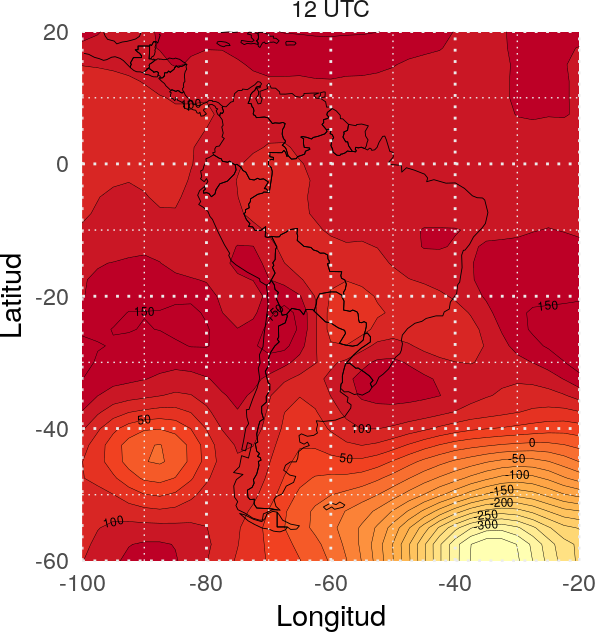
\includegraphics{Tesis_files/figure-latex/hgt-caso1-1} 

}

\caption{Altura geopotencial en 1000 hPa para las 00 y las 12 UTC del 14 de enero de 2016 (Caso 1). Datos de Reanálisis NCEP (NOAA/OAR/ESRL PSD - Kalnay et al., 1995). \label{hgt-caso1}}\label{fig:hgt-caso1}
\end{figure}

\begin{figure}

{\centering 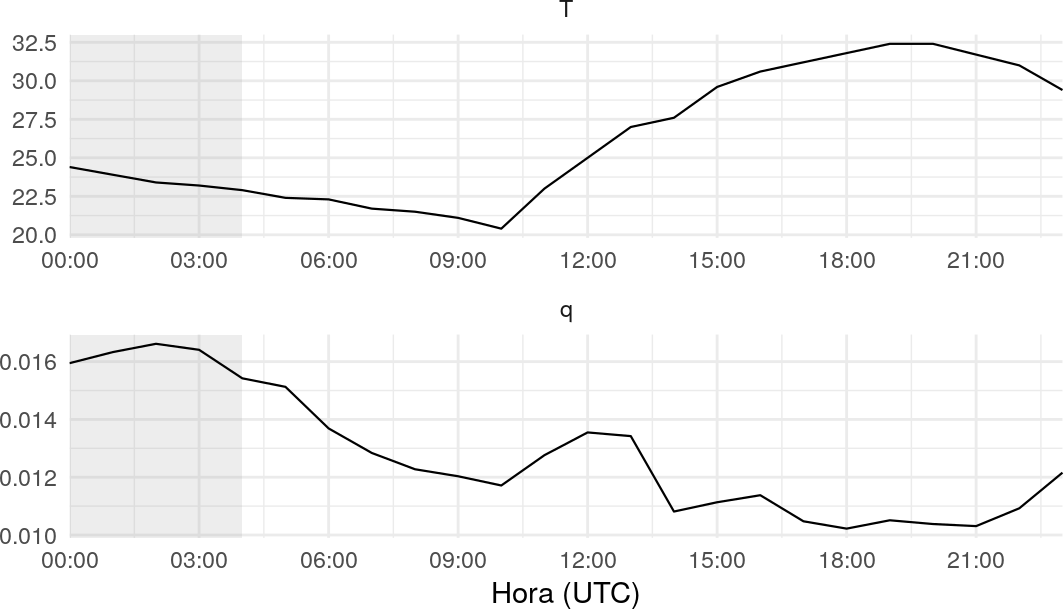
\includegraphics{Tesis_files/figure-latex/meteo-caso1-1} 

}

\caption{Variables de superficie observadas por la estación meteorológica Paraná el 14 de enero de 2016. La región sombreada corresponde a al período donde se observa nubosidad (ver texto). Datos Servicio Meteorológico Nacional. \label{meteo1}}\label{fig:meteo-caso1}
\end{figure}

\subsection{Caso 2: 21 de enero de
2016}\label{caso-2-21-de-enero-de-2016}

El caso 2 comprende el período entre las 00 UTC del 21 de enero a las 00
UTC del 22 de enero de 2016. A escala regional a las 00 UTC (Figura
\ref{hgt-caso2}) se observó un anticiclón ubicado sobre el océano
Atlántico frente a la costa de Argentina, mientrás que en el centro del
país se observó una región de baja presión. De acuerdo a los datos de la
estación meteorológica en las primeras horas del día el viento estuvo en
calma y llegando a los 2 m/s en algunos momentos. La dirección
predominante fue del E y SE en algnas horas. En cuanto a la nubosidad,
en las primeras cuatro horas se observó nubosidad de tipo
\emph{cirrostratus} que no cubrió la totalidad del cielo en ningún
momento. No no afectó el descenso de temperatura durante las horas
nocturnas.

Posteriormente a las 12 UTC del mismo día el anticiclón se debilitó y se
desplazó hacia el noreste. El viento en superfie fue de predominante del
N a partir de esa hora con máximos de hasta 5.5 m/s. Esta situación
generó un aumento de la humedad específica proveniente del norte con un
máximo luego de las 14 UTC. Entre las 09 y las 16 UTC se observó
nubosidad tipo \emph{cirro} que no llegó a cubrir la totalidad del
cielo. Esta nubosidad no afectó de manera observarble la temperatura en
superficie que llegó a 35.4°C. En las observaciones del radar no se vió
nubosidad en las inmediaciones.

\begin{figure}

{\centering \includegraphics{Tesis_files/figure-latex/hgt-caso2-1} 

}

\caption{Altura geopotencial en 1000 hPa para las 00 y las 12 UTC del 21 de enero de 2016 (Caso 2). Datos de Reanálisis NCEP (NOAA/OAR/ESRL PSD - Kalnay et al., 1995). \label{hgt-caso2}}\label{fig:hgt-caso2}
\end{figure}

\begin{figure}

{\centering \includegraphics{Tesis_files/figure-latex/meteo-caso2-1} 

}

\caption{Variables de superficie observadas por la estación meteorológica Paraná el 21 de enero de 2016. La región sombreada corresponde a al período donde se observa nubosidad (ver texto). Datos Servicio Meteorológico Nacional. \label{meteo2}}\label{fig:meteo-caso2}
\end{figure}

\subsection{Caso 3: 23 de enero de
2016}\label{caso-3-23-de-enero-de-2016}

El caso 3 abarca el periodo de las 00 UTC del 23 de enero a las 00 UTC
del 24 de enero de 2016. A nivel regional el campo de altura
geopotencial en 1000 hPa muestró una región de baja presión en el centro
del país (Figura \ref{hgt-caso3}) que fue desplazándose hacia en NE a lo
largo del periodo. Esta configuración puede ser asociada con vientos del
N en la región de Paraná, lo que se confirma con los datos de viento
registrados en la estación meteorológica débiles a moderados (entre 1.5
y 5 m/s).

Entre las 06 y 09 UTC se observó nubosidad que cubrió dos octavos del
cielo de tipo \emph{altocumulus} semitransparentes. Si bien esta
nubosidad se observó alejada de radar (a más de 60 km hacia el NE),
puede ser la causa del estancamiento de la temperatura en la estación
meteorológica durante ese período pero que luego siguió descendiendo al
desaparecer la nubosidad. El máximo de humedad específica observado
durante las horas nocturnas pudo deberse al transporte de humedad debido
al viento del N y del NNE (Figura \ref{meteo3}).

A las 12 UTC el centro de baja presión fue reemplazado por un anticiclón
que se ubicó al sur de la provincia del Buenos Aires y sobre la costa
del océano Atlántico. En superficie se registró viento del NO y O con un
máximo de 5.5 m/s). Entre las 14 y las 17 UTC se registró nubosidad alta
de tipo \emph{cirrus} en forma de filamentos y bandas que no cubrieron
la totalidad del cielo en ningún momento. El aumento diurno de la
temperatura fue constante hasta llegar a una máxima de 37.2°C a las 20
UTC.

\begin{figure}

{\centering \includegraphics{Tesis_files/figure-latex/hgt-caso3-1} 

}

\caption{Altura geopotencial en 1000 hPa para las 00 y las 12 UTC del 23 de enero de 2016 (Caso 3). Datos de Reanálisis NCEP (NOAA/OAR/ESRL PSD - Kalnay et al., 1995). \label{hgt-caso3}}\label{fig:hgt-caso3}
\end{figure}

\begin{figure}

{\centering \includegraphics{Tesis_files/figure-latex/meteo-caso3-1} 

}

\caption{Variables de superficie observadas por la estación meteorológica Paraná el 23 de enero de 2016. La región sombreada corresponde a al período donde se observa nubosidad (ver texto). Datos Servicio Meteorológico Nacional. \label{meteo3}}\label{fig:meteo-caso3}
\end{figure}

\section{Análisis de las observaciones de radar procesadas con
VAD}\label{analisis-de-las-observaciones-de-radar-procesadas-con-vad}

\subsection{Magnitud y velocidad del
viento}\label{magnitud-y-velocidad-del-viento}

Analisis de la magnitud y velocidad del viento a lo largo del tiempo y
para cada caso. Ver Los errores, zonas sin datos, datos en superficie.
Luego características generales, evolución día-noche, máximo nocturno
(que da pie al LLJ luego), rotación con la altura.

\begin{figure}
\subfloat[Magnitud del viento. \label{caso1-spd}\label{fig:campo-caso11}]{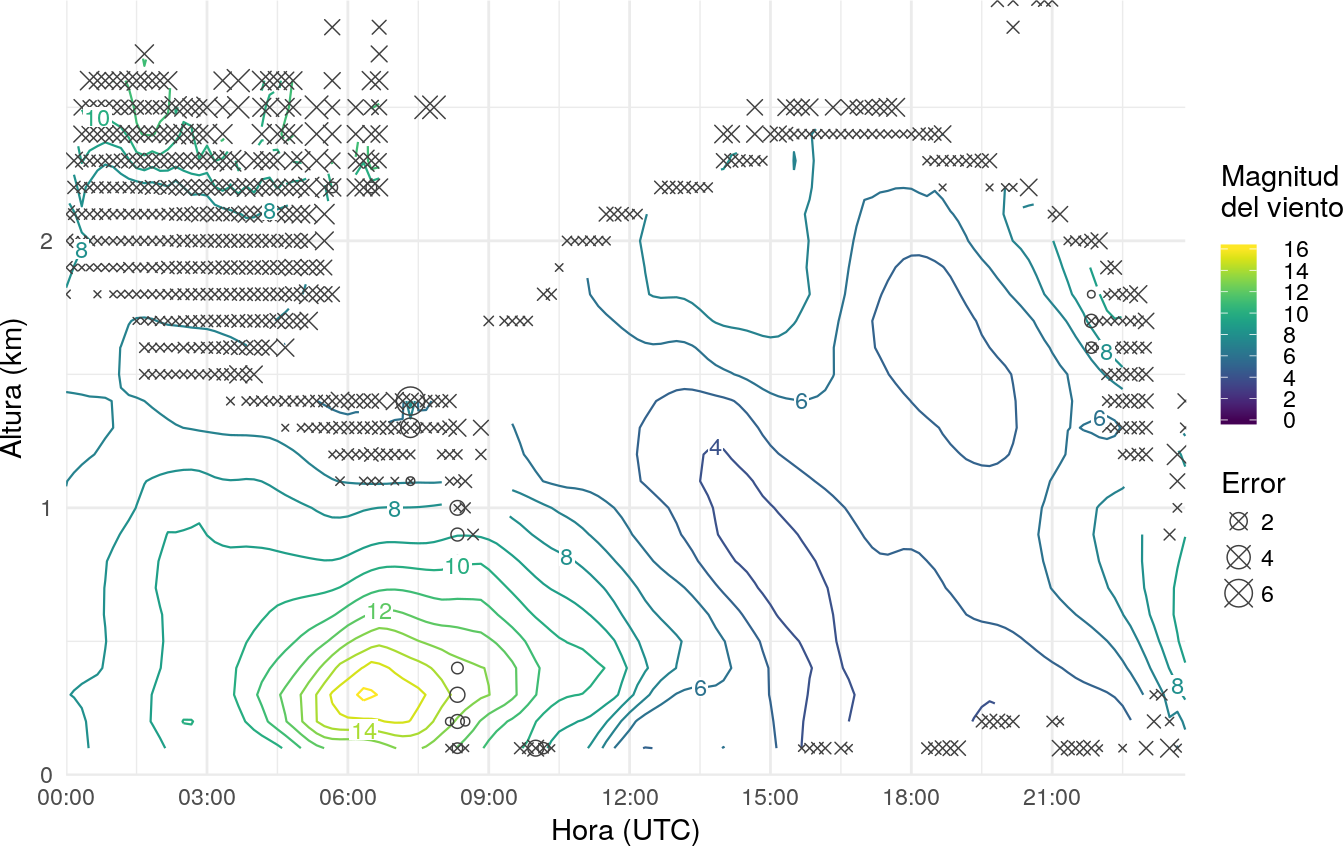
\includegraphics{Tesis_files/figure-latex/campo-caso1-1} }\newline\subfloat[Dirección. \label{caso1-dir}\label{fig:campo-caso12}]{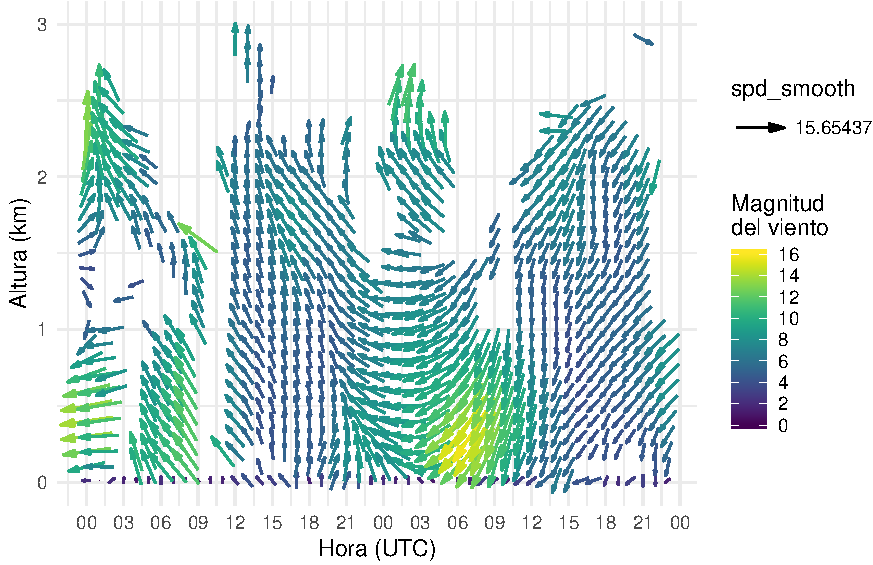
\includegraphics{Tesis_files/figure-latex/campo-caso1-2} }\caption{Magnitud y dirección del viento  correspondiente al Caso 1 (14/01/2016) observados por el radar y procesados con VAD. En el caso de la magnitud del viento se muestra además los errores calculados ($rmse_1$ y $rmse_2$) cuando superan los 0.5 m/s. \label{campo-caso1}}\label{fig:campo-caso1}
\end{figure}

\begin{figure}
\subfloat[Magnitud del viento. \label{caso2-spd}\label{fig:campo-caso21}]{\includegraphics{Tesis_files/figure-latex/campo-caso2-1} }\newline\subfloat[Dirección. \label{caso2-dir}\label{fig:campo-caso22}]{\includegraphics{Tesis_files/figure-latex/campo-caso2-2} }\caption{Magnitud y dirección del viento  correspondiente al Caso 2 (21/01/2016) observados por el radar y procesados con VAD. En el caso de la magnitud del viento se muestra además los errores calculados ($rmse_1$ y $rmse_2$) cuando superan los 0.5 m/s. \label{campo-caso2}}\label{fig:campo-caso2}
\end{figure}

\begin{figure}
\subfloat[Magnitud del viento. \label{caso3-spd}\label{fig:campo-caso31}]{\includegraphics{Tesis_files/figure-latex/campo-caso3-1} }\newline\subfloat[Dirección. \label{caso3-dir}\label{fig:campo-caso32}]{\includegraphics{Tesis_files/figure-latex/campo-caso3-2} }\caption{Magnitud y dirección del viento  correspondiente al Caso 3 (23/01/2016) observados por el radar y procesados con VAD. En el caso de la magnitud del viento se muestra además los errores calculados ($rmse_1$ y $rmse_2$) cuando superan los 0.5 m/s. \label{campo-caso3}}\label{fig:campo-caso3}
\end{figure}

Con esta figura ver las características del perfil del viento para el
caso nocturno y el caso diurno. También el máximo asociado al LLJ y más
adelante el criterio de Bonner.

\begin{figure}

{\centering 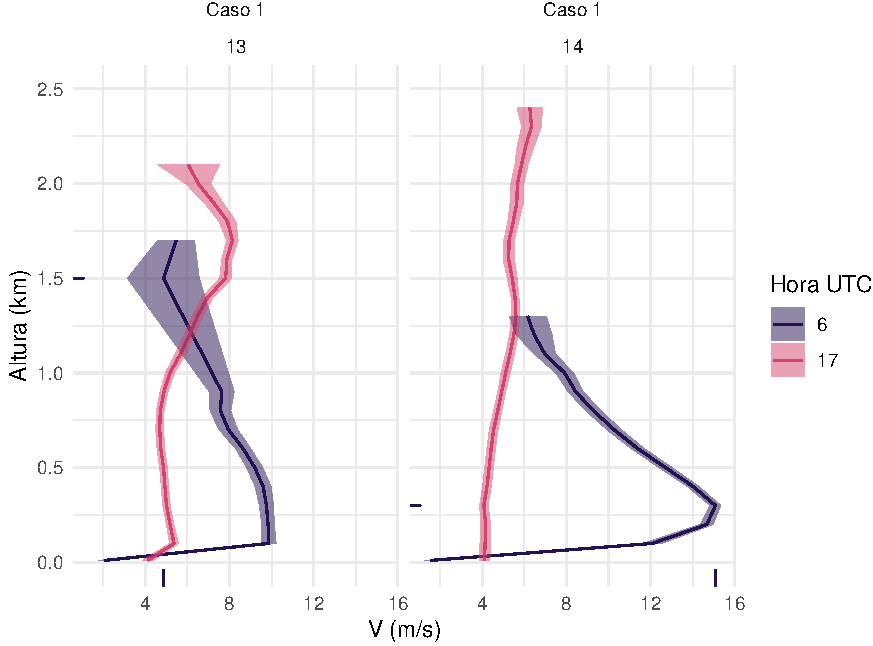
\includegraphics{Tesis_files/figure-latex/perfiles-1} 

}

\caption{Perfil de viento observado por el radar a las 0600 y las 1700 UTC y el $rmse_2$ en cada punto (sombreado) para los tres casos. Las marcas en los ejes indican la magnitud del viento máxima y mínima y la altura a la que ocurren. Los valores en superficie fueron obtenidos a partir de los datos del la estación meteorógica Paraná Aero. \label{perfiles-horarios}}\label{fig:perfiles}
\end{figure}

\subsection{Características de la capa límite
planetaria}\label{caracteristicas-de-la-capa-limite-planetaria}

\subsubsection{Altura de la capa límite y
turbulencia}\label{altura-de-la-capa-limite-y-turbulencia}

Altura de la clp con reflectividad. Ver ese dobe tope durante el día y
la noche (tope de la capa residual?). Ver que hay de interesante en cada
caso.

\begin{figure}

{\centering \subfloat[Caso 1. \label{dbz-1}\label{fig:pblh-dbz1}]{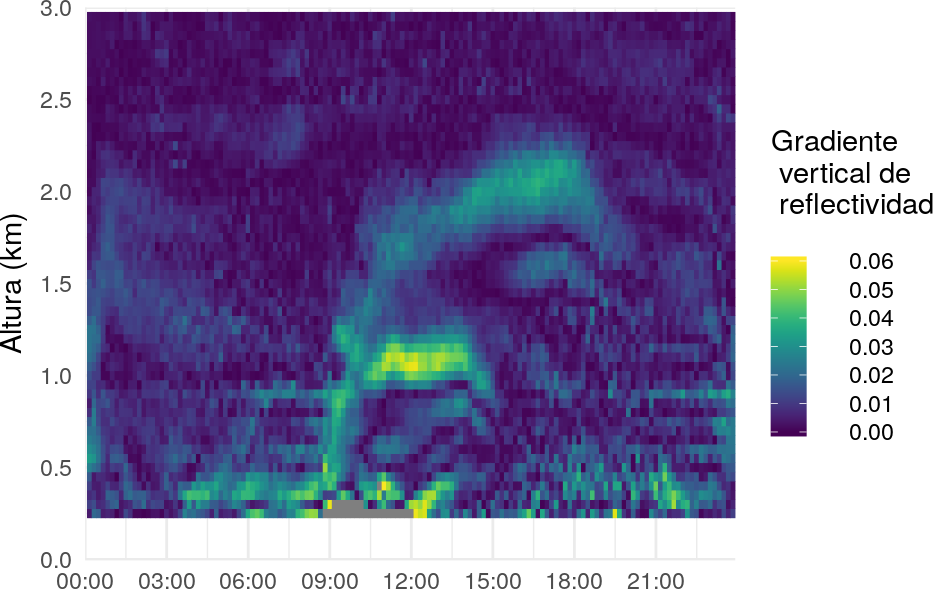
\includegraphics{Tesis_files/figure-latex/pblh-dbz-1} }\newline\subfloat[Caso2. \label{dbz-2}\label{fig:pblh-dbz2}]{\includegraphics{Tesis_files/figure-latex/pblh-dbz-2} }\newline\subfloat[Caso 3. \label{dbz-3}\label{fig:pblh-dbz3}]{\includegraphics{Tesis_files/figure-latex/pblh-dbz-3} }

}

\caption{Valor absoluto del gradiente vertical de dBZ en función de la altura y el tiempo. \label{pblh-dbz}}\label{fig:pblh-dbz}
\end{figure}

La altura de la capa límite se empalma con las caractersíticas
turbulentas, acá no tengo mucho pero puedo usar el número de Richardson,
la cortante y la comparación con la otra forma de estimar la altura de
la CLP.

\begin{figure}
\subfloat[Altura de la capa estable \label{h-vad}\label{fig:estable-vad1}]{\includegraphics{Tesis_files/figure-latex/estable-vad-1} }\newline\subfloat[Cortante ($u_{máx}/z_{máx}$) \label{cortante-vad}\label{fig:estable-vad2}]{\includegraphics{Tesis_files/figure-latex/estable-vad-2} }\newline\subfloat[Número de Richardson \label{ri}\label{fig:estable-vad3}]{\includegraphics{Tesis_files/figure-latex/estable-vad-3} }\caption{Series de tiempo de la altura de la capa límite, cortante vertical y el número de Richarsdon en la capa estable nocturna para todos los casos de estudio. En a) y b) se muestra solo el período donde se observa el LLJ, en c) el período en cada caso se encuentra sombreado. \label{estable-vad}}\label{fig:estable-vad}
\end{figure}

Ekman, ojo que hay que tener en cuenta la altura de la clp, por arriba
no vale.

\begin{figure}

{\centering 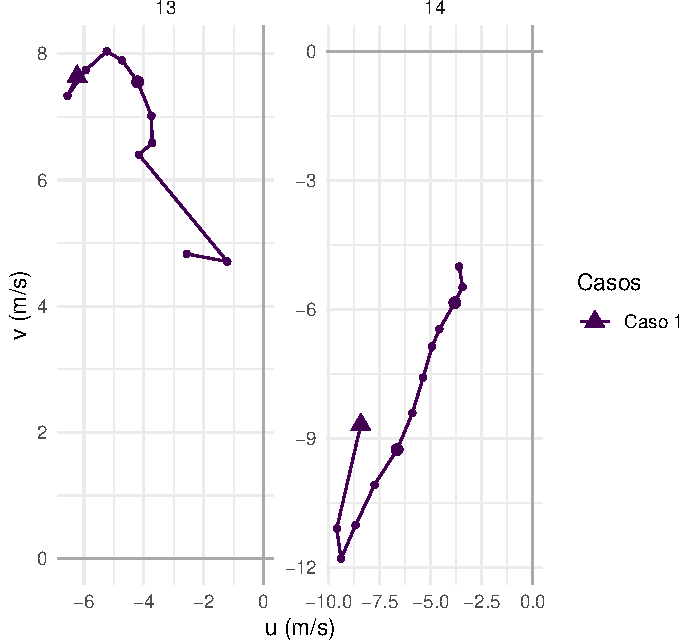
\includegraphics{Tesis_files/figure-latex/hodografa-horaria-1} 

}

\caption{Variación del vector del viento en función de la altura entre 100 y 3000 metros, para cada caso de estudio observada por el radar a las 0600 UTC. El triángulo marca el nivel inferior y los círculos grandes se ubican cada 500 metros. \label{hodografa-h}}\label{fig:hodografa-horaria}
\end{figure}

\subsubsection{Oscilación inercial y
LLJ}\label{oscilacion-inercial-y-llj}

Criterio de bonner, modelos de oscilación inercial propuesto por otros
autores, giro de la hodógrafa en e tiempo. Periodo inercial.

\begin{figure}

{\centering \subfloat[Datos observados en la estación meteorológica. \label{hodo-nivel1}\label{fig:hodografa-nivel1}]{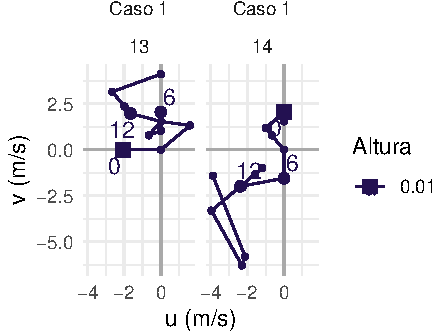
\includegraphics{Tesis_files/figure-latex/hodografa-nivel-1} }\newline\subfloat[Datos observados por el radar. \label{hodo-nivel2}\label{fig:hodografa-nivel2}]{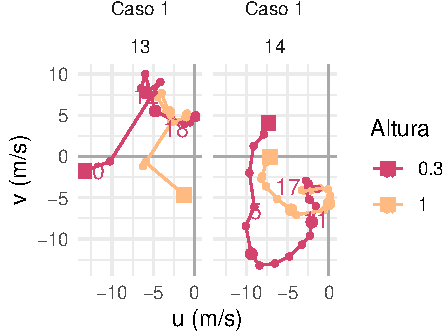
\includegraphics{Tesis_files/figure-latex/hodografa-nivel-2} }

}

\caption{Variación del vector del viento en función del tiempo para tres niveles. Cada circulo representa un valor horario (con circulos más grandes cada 6 horas) y el cuadrado marca el primer tiempo (0000 UTC). \label{hodografa-n}}\label{fig:hodografa-nivel}
\end{figure}

\section{Analisis de las simulaciones y comparación con observaciones de
radar}\label{analisis-de-las-simulaciones-y-comparacion-con-observaciones-de-radar}

\subsection{Magnitud y dirección del
viento}\label{magnitud-y-direccion-del-viento}

Descripción general de la magnitud y la dirección del viento en cada
simulación y como se parece a las observaciones. Bias, correlación y
otros errores. A resolver: como trabajar con la dirección del viento.

\begin{figure}

{\centering 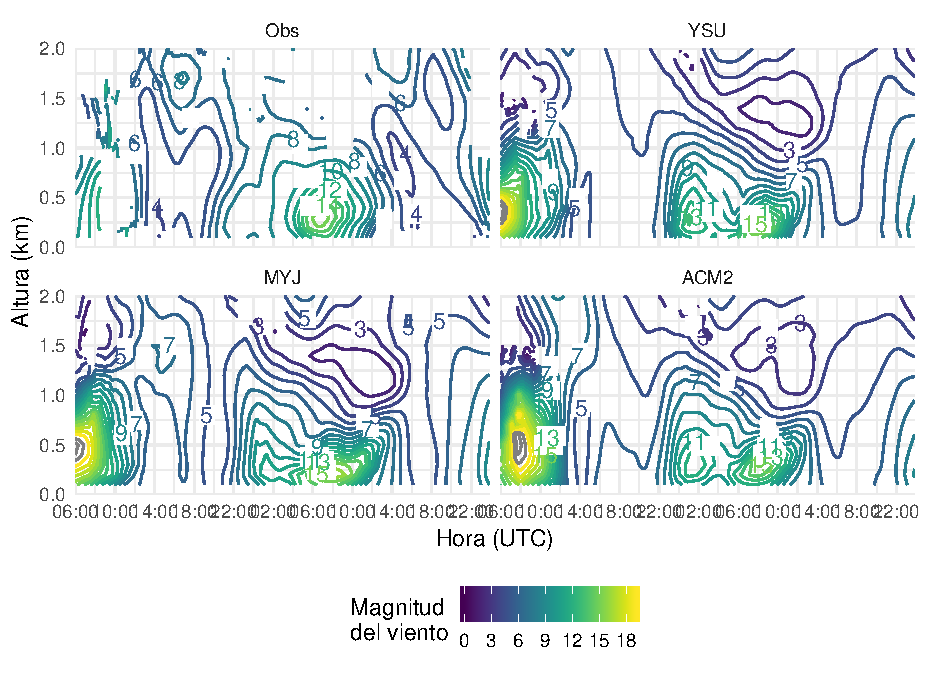
\includegraphics{Tesis_files/figure-latex/vad-modelo-spd-1} 

}

\caption{Magnitud del viento observada por el radar (Obs) y simulada por el modelo WRF utilizando distintos esquemas de CLP para el Caso 1 (14/01/2016) y posteriormente procesados con VAD. \label{modelo-spd}}\label{fig:vad-modelo-spd}
\end{figure}

\begin{figure}

{\centering 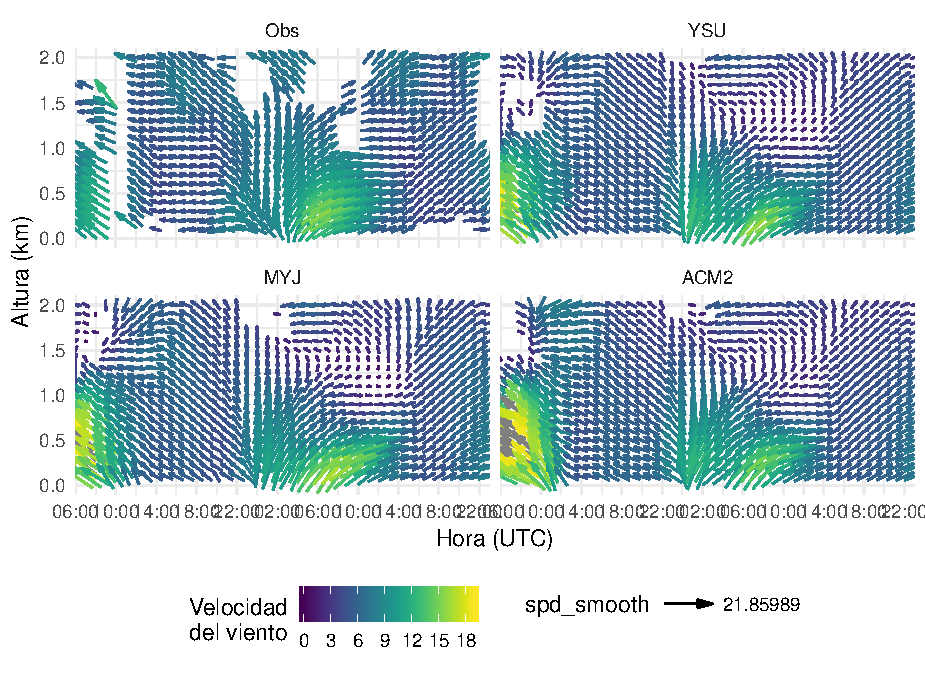
\includegraphics{Tesis_files/figure-latex/vad-modelo-dir-1} 

}

\caption{Dirección del viento observada por el radar(Obs) y simulada por el modelo WRF utilizando distintos esquemas de CLP para el Caso 1 (14/01/2016) y posteriormente procesados con VAD. \label{modelo-dir}}\label{fig:vad-modelo-dir}
\end{figure}

\begin{figure}
\subfloat[Magnitud del viento \label{dif-spd}\label{fig:diferencia1}]{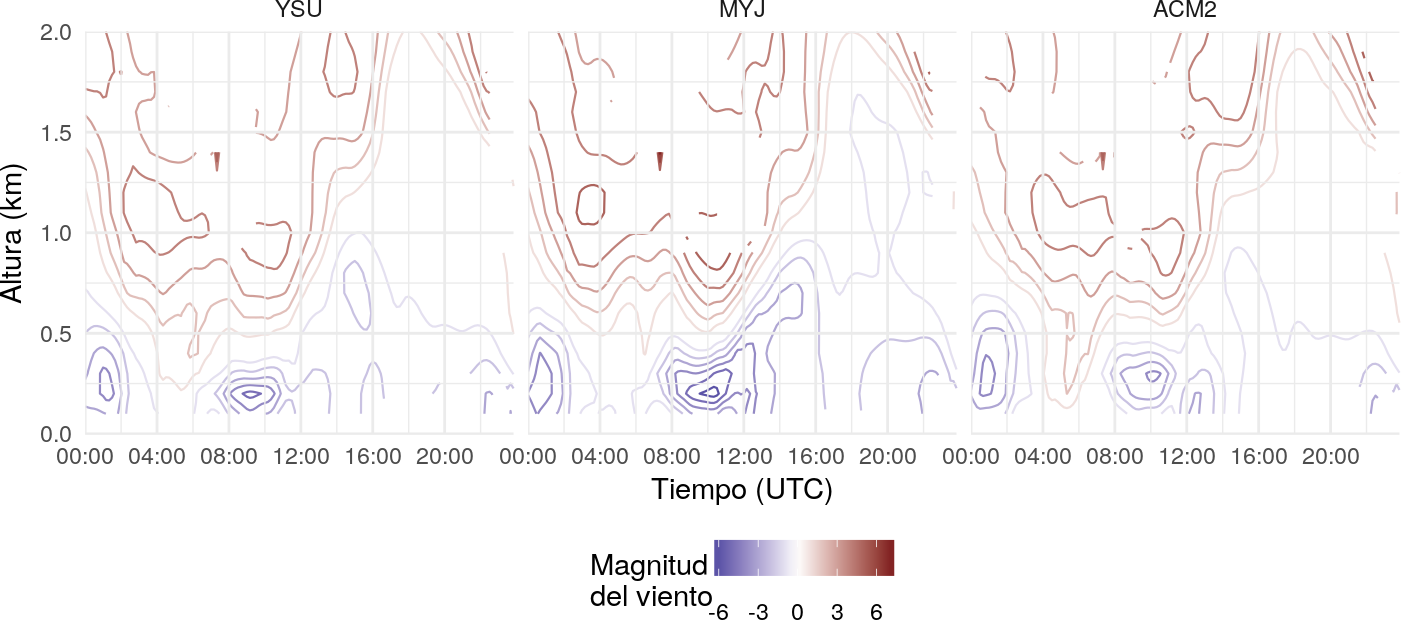
\includegraphics{Tesis_files/figure-latex/diferencia-1} }\subfloat[Ángulo de la dirección del viento \label{dif-dir}\label{fig:diferencia2}]{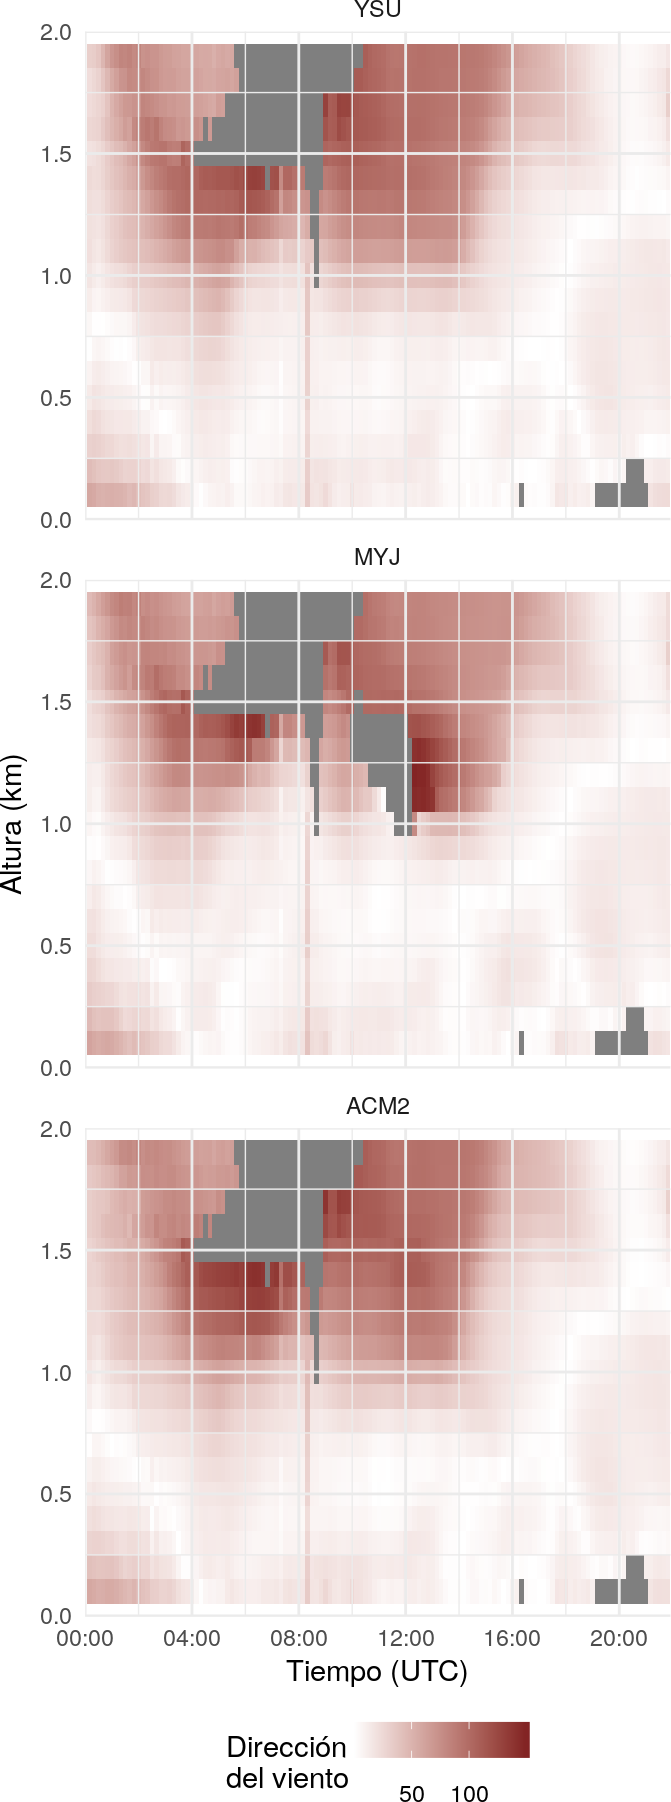
\includegraphics{Tesis_files/figure-latex/diferencia-2} }\caption{Diferencia entre las observaciones y cada simulación  correspondiente al Caso 1. \label{dif}}\label{fig:diferencia}
\end{figure}

\begin{figure}

{\centering \subfloat[bias. \label{bias-spd}\label{fig:err-spd1}]{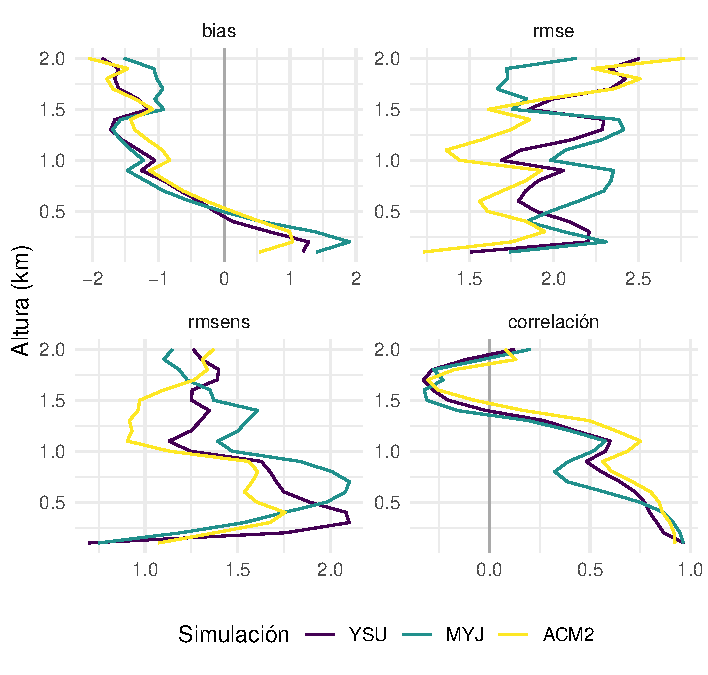
\includegraphics{Tesis_files/figure-latex/err-spd-1} }\subfloat[rmse. \label{rmse-spd}\label{fig:err-spd2}]{\includegraphics{Tesis_files/figure-latex/err-spd-2} }\newline\subfloat[rmsens. \label{rmsens-spd}\label{fig:err-spd3}]{\includegraphics{Tesis_files/figure-latex/err-spd-3} }\subfloat[correlación. \label{cor-spd}\label{fig:err-spd4}]{\includegraphics{Tesis_files/figure-latex/err-spd-4} }

}

\caption{Errores calculados para la estimación de la velocidad del viento (m/s) con cada simulación en función de la altura y la correlación. \label{err-spd}}\label{fig:err-spd}
\end{figure}

\begin{table}

\caption{\label{tab:err-tabla}Comparación entre las simulaciones y las observaciones de radar a partir de distintos errores}
\centering
\begin{tabular}[t]{lrrrrrrrr}
\toprule
\multicolumn{1}{c}{ } & \multicolumn{4}{c}{Velocidad} & \multicolumn{4}{c}{Dirección} \\
\cmidrule(l{2pt}r{2pt}){2-5} \cmidrule(l{2pt}r{2pt}){6-9}
caso & bias & rmse & rmsens & correlación & bias & rmse & rmsens & correlación\\
\midrule
YSU & -0.8484 & 2.3088 & 2.1254 & 0.6814 & -24.7264 & 43.8039 & 35.4133 & 0.5459\\
MYJ & -0.5639 & 2.5587 & 2.4851 & 0.6332 & -21.8190 & 41.6008 & 34.7102 & 0.5447\\
ACM2 & -1.0089 & 2.3356 & 2.0733 & 0.7112 & -25.7172 & 45.4811 & 36.7295 & 0.5270\\
\bottomrule
\end{tabular}
\end{table}

\subsection{Características de la capa límite
planetaria}\label{caracteristicas-de-la-capa-limite-planetaria-1}

\subsubsection{Oscilacion inercial y
LLJ}\label{oscilacion-inercial-y-llj-1}

\begin{figure}

{\centering 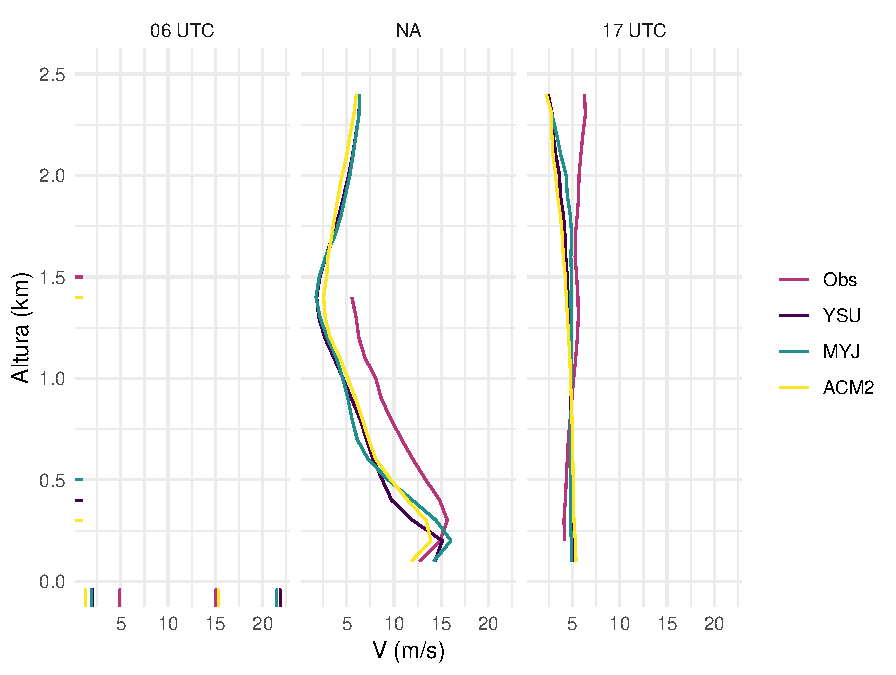
\includegraphics{Tesis_files/figure-latex/perfiles-mod-1} 

}

\caption{Perfil de viento observado por el radar a las 0600 y las 1700 UTC y perfiles simulados por el modelo para los mismos momentos. Las marcas en los ejes indican la magnitud del viento máxima y mínima y la altura a la que ocurren. \label{perfiles-modelo}}\label{fig:perfiles-mod}
\end{figure}

\begin{figure}

{\centering 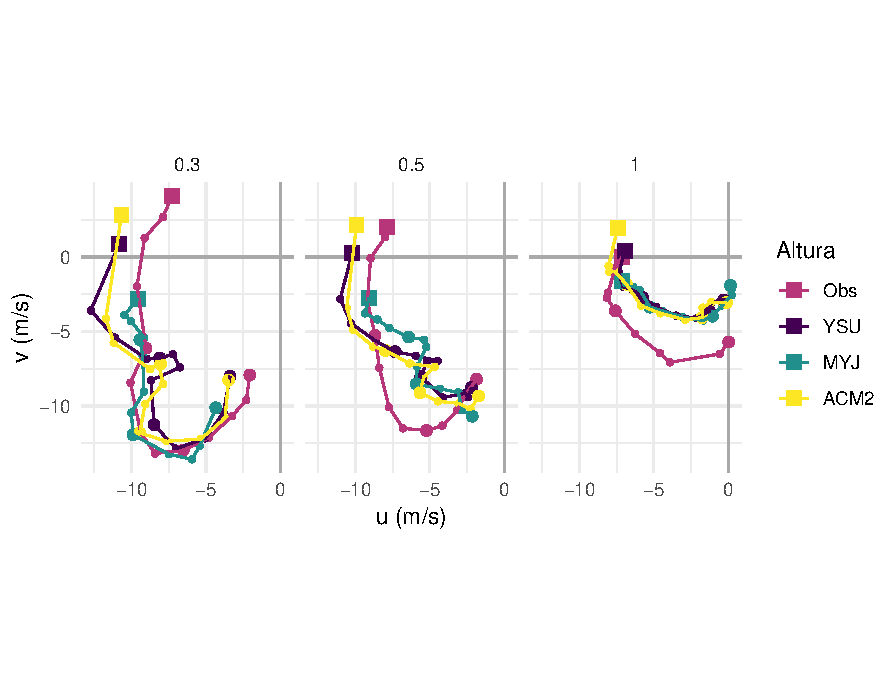
\includegraphics{Tesis_files/figure-latex/hodografa-wrf-1} 

}

\caption{Variación del vector del viento en función del tiempo para tres niveles. Cada circulo representa un valor horario (con circulos más grandes cada 4 horas) y el cuadrado marca el primer tiempo (0000 UTC). \label{hodografa-wrf}}\label{fig:hodografa-wrf}
\end{figure}

\subsubsection{Análisis de la homogeneidad espacial en las variables de
estabilidad}\label{analisis-de-la-homogeneidad-espacial-en-las-variables-de-estabilidad}

Para determinar la validez del promedio espacial de una variable en el
dominio en estudio es importante analizar la variabilidad de la misma
espacial y temporalmente.

Se utilizó la Longitud de Monin-Obukhov (\(L\)) para analizar la
homogeneidad calculando el procentaje de veces que el valor local tenía
signo distinto a la moda calculada para todo el dominio y cada tiempo de
simulación. Esto es importante ya que el signo de \(L\) marca la
diferencia entre el regimen estable y el regimen inestable y por lo
tanto debe mantenerse en el dominio en cada período.

En la Figura \ref{L-espacial} se muestra el porcentaje de veces que el
valor de \(L\) en cada punto de grilla tiene signo distinto a la moda
calculada en todo el dominio y el período analizado. Se observa que que
existen regiones donde el signo de \(L\) es distinto a la moda del
dominio más del 40\% de las veces. Esto puede estar relacionado la
variación de la altura del terreno (Figura \ref{topografia}) o a la
presencia del río y zonas con suelos saturados donde los flujos
verticales de calor latente (\(F_{\theta}\)) pueden tener un
comportamiento contrario al suelo seco. Esto último se observa en la
Figura \ref{L-espacial}, donde se muestra que las regiones donde el
porcentaje de veces que el valor de \(F_{\theta}\) tiene un signo
distinto a la moda es alto coincide con las regiones donde se encuentra
el río y los valores de \(L\) anómalos.

\begin{figure}

{\centering \includegraphics{Tesis_files/figure-latex/L-espacial-1} 

}

\caption{Porcentaje de veces que el valor local de L (a) y el flujo vertical de calor (b) tiene signo distinto a la moda del dominio calculada en todo el periodo analizado. Se muestran los valores mayores al 5\% (colores) y topografía del dominio (contornos). Datos de la simulación YSU. \label{L-esp}}\label{fig:L-espacial}
\end{figure}

Por lo anterior se decidió centrar el análsis de las variables asociadas
a la CLP en el punto de grilla más cercano al radar, que además no
presenta gran variabilidad respecto de la zona circundante.

\begin{figure}

{\centering 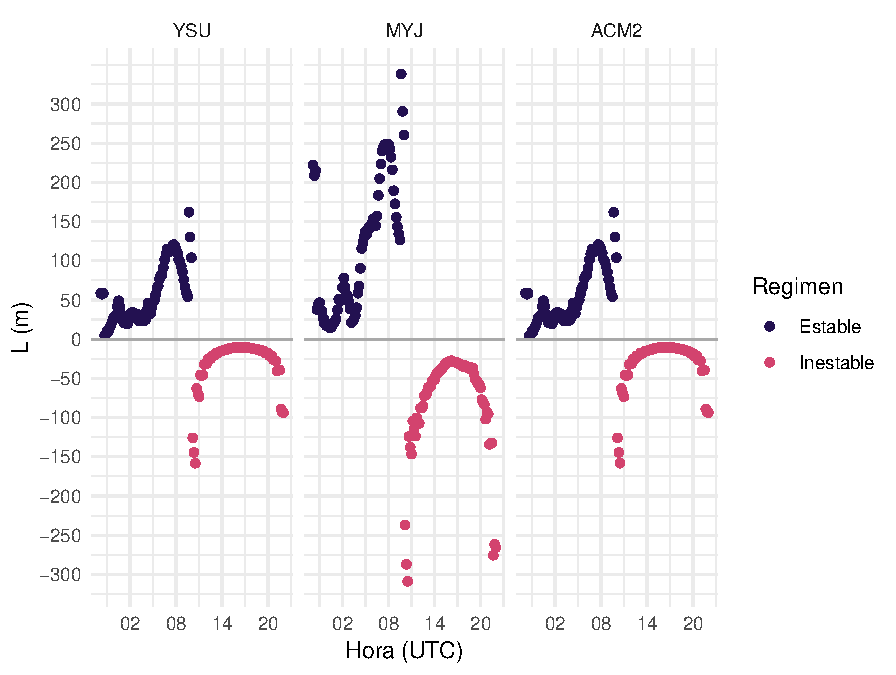
\includegraphics{Tesis_files/figure-latex/L-parm-1} 

}

\caption{Longitud de Monin Obukhov (m) en función del tiempo, para cada simulación. \label{L-param}}\label{fig:L-parm}
\end{figure}

\subsubsection{Altura de la capa
límite}\label{altura-de-la-capa-limite-1}

\begin{figure}

{\centering \subfloat[Estimada directamente por cada esquema de CLP. \label{pblh}\label{fig:pblh-wrf1}]{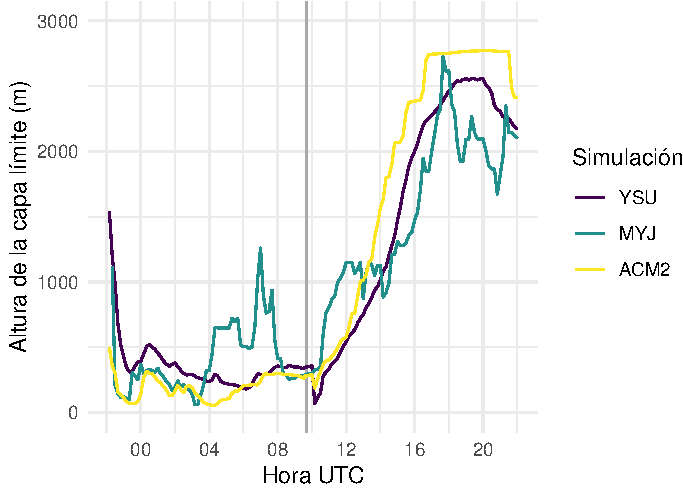
\includegraphics{Tesis_files/figure-latex/pblh-wrf-1} }\newline\subfloat[Comparación entre la altura calculada por cada esquema (linea) y la estimada a partir de la altura del viento máximo (puntos) sólo período estable. \label{pblh-spd}\label{fig:pblh-wrf2}]{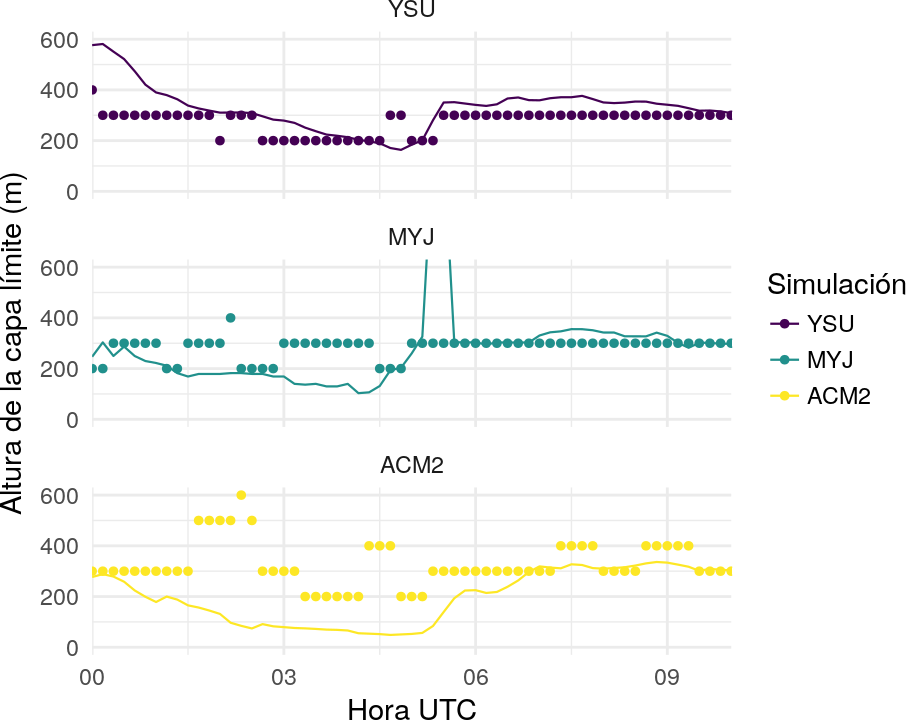
\includegraphics{Tesis_files/figure-latex/pblh-wrf-2} }

}

\caption{Altura de la capa límite en cada simulación. \label{pblh-wrf}}\label{fig:pblh-wrf}
\end{figure}

\begin{figure}

{\centering \includegraphics{Tesis_files/figure-latex/dbz-wrf-1} 

}

\caption{Valor absoluto del gradiente vertical de dBZ en función de la altura y el tiempo. \label{pblh-dbz}}\label{fig:dbz-wrf}
\end{figure}

\subsubsection{Coeficientes de difusividad
turbulenta}\label{coeficientes-de-difusividad-turbulenta-1}

\begin{figure}

{\centering \subfloat[$K_h* = K_h/khu_*$ \label{kh-norm}\label{fig:k_norm1}]{\includegraphics{Tesis_files/figure-latex/k_norm-1} }\newline\subfloat[$K_m* = K_m/khu_*$ \label{km-norm}\label{fig:k_norm2}]{\includegraphics{Tesis_files/figure-latex/k_norm-2} }

}

\caption{Coeficiente de difusividad normalizados calculados a partir de los modelos propuestos por Ulke 2000 y promediados sobre en período estable (izquierda) y el período inestable (derecha) de la capa límite. \label{kh-ulke}}\label{fig:k_norm}
\end{figure}

\begin{figure}

{\centering \includegraphics{Tesis_files/figure-latex/pr-1} 

}

\caption{Variación del número de Prandtl calculado a partir del modelo propuesto por Ulke 2000 con las variables de cada simulación y promediado en cada periodo. \label{Pr}}\label{fig:pr}
\end{figure}

\begin{table}

\caption{\label{tab:tabla-clp}Parámetros característicos de la capa límite para cada simulación y regimen, promediados para todo el periodo y todo el perfil (en los casos que corresponda).}
\centering
\begin{tabular}[t]{llrrrrr}
\toprule
Simulación & Regimen & $\overline{h}$\textsuperscript{1} & $\overline{L}$\textsuperscript{2} & $\overline{u*}$\textsuperscript{3} & $\overline{Pr}$\textsuperscript{4} & $h/L$\\
\midrule
YSU & Estable & 368.67 & 45.30 & 0.2911 & 1.33 & 8.14\\
YSU & Inestable & 1563.14 & -35.07 & 0.6020 & 0.26 & -44.57\\
MYJ & Estable & 273.63 & 84.67 & 0.3134 & 1.32 & 3.23\\
MYJ & Inestable & 1569.49 & -95.79 & 0.6198 & 0.34 & -16.38\\
ACM2 & Estable & 199.32 & 45.30 & 0.2697 & 1.33 & 4.40\\
ACM2 & Inestable & 1871.88 & -35.07 & 0.6055 & 0.26 & -53.37\\
\bottomrule
\multicolumn{7}{l}{\textsuperscript{1} Altura de la CLP promediada.}\\
\multicolumn{7}{l}{\textsuperscript{2} Longitud de Monin Obukhov promediada.}\\
\multicolumn{7}{l}{\textsuperscript{3} Velocidad de fricción promediada.}\\
\multicolumn{7}{l}{\textsuperscript{4} Número de Prandtl promediado.}\\
\end{tabular}
\end{table}

\begin{figure}

{\centering \subfloat[Calor $K_h$ ($m^2/s$). \label{kh-wrf}\label{fig:k_ulke_wrf1}]{\includegraphics{Tesis_files/figure-latex/k_ulke_wrf-1} }\newline\subfloat[Moviento $K_m$ ($m^2/s$). \label{km-wrf-ulke}\label{fig:k_ulke_wrf2}]{\includegraphics{Tesis_files/figure-latex/k_ulke_wrf-2} }

}

\caption{Coeficientes de difusividad promediados para todo el período estable (izquierda) y el período inestable (derecha) de la capa límite en todas las simulaciones. \label{kh_wrf}}\label{fig:k_ulke_wrf}
\end{figure}

\chapter{Conclusiones}\label{conclusiones}

\chapter*{Referencias}\label{referencias}
\addcontentsline{toc}{chapter}{Referencias}

\hypertarget{refs}{}
\hypertarget{ref-Acevedo2014}{}
Acevedo, O.C., Costa, F.D., Oliveira, P.E.S., Puhales, F.S., Degrazia,
G.A., y Roberti, D.R., 2014. The Influence of Submeso Processes on
Stable Boundary Layer Similarity Relationships. Journal of the
Atmospheric Sciences, 71, 1, 207-225.

\hypertarget{ref-Amante2009}{}
Amante, C., y Eakins, B., 2009. ETOPO1 1 Arc-Minute Global Relief Model:
Procedures, Data Sources and Analysis.

\hypertarget{ref-Banks2016}{}
Banks, R.F., Tiana-Alsina, J., Baldasano, J.M., Rocadenbosch, F.,
Papayannis, A., Solomos, S., y Tzanis, C.G., 2016. Sensitivity of
boundary-layer variables to PBL schemes in the WRF model based on
surface meteorological observations, lidar, and radiosondes during the
HygrA-CD campaign. Atmospheric Research, 176-177, 185-201.

\hypertarget{ref-Berri2012}{}
Berri, G.J., Nuin, J.S.G., Sraibman, L., y Bertossa, G., 2012.
Verification of a Synthesized Method for the Calculation of Low-Level
Climatological Wind Fields Using a Mesoscale Boundary-Layer Model.
Boundary-Layer Meteorology, 142, 2, 329-337.

\hypertarget{ref-Blackadar1957}{}
Blackadar, A.K., 1957. Boundary Layer Wind Maxima and Their Significance
for the Growth of Nocturnal Inversions. Bulletin of the American
Meteorological Society, 38, 5, 283-290.

\hypertarget{ref-Bonner1968}{}
Bonner, W.D., 1968. Monthly Weather Review Climatology of the Low Level
Jet. Monthly Weather Review, 96, 12, 833-850.

\hypertarget{ref-Bousquet2008}{}
Bousquet, O., Montmerle, T., y Tabary, P., 2008. Using operationally
synthesized multiple-Doppler winds for high resolution horizontal wind
forecast verification. Geophysical Research Letters, 35, 10, 1-6.

\hypertarget{ref-Browning1968}{}
Browning, K.A., y Wexler, R., 1968. The Determination of Kinematic
Properties of a Wind Field Using Doppler Radar. Journal of Applied
Meteorology, 7, 1, 105-113.

\hypertarget{ref-Chandra2010}{}
Chandra, A.S., Kollias, P., Giangrande, S.E., y Klein, S.A., 2010.
Long-term observations of the convective boundary layer using insect
radar returns at the SGP ARM climate research facility. Journal of
Climate, 23, 21, 5699-5714.

\hypertarget{ref-Cleveland1979}{}
Cleveland, W.S., 1979. Robust locally weighted regression and smoothing
scatterplots. J. Am. Stat. Assoc.74: 829-836. Journal of the American
Statistical Association, 74, 368, 829-836.

\hypertarget{ref-Collis2016}{}
Collis, S., 2016. Py-ART The Python ARM Radar Toolkit.
(http://arm-doe.github.io/pyart/).

\hypertarget{ref-Dixon2010}{}
Dixon, M., 2010. Radx C++ library - NCAR Earth Observing Laboratory.
(https://www.eol.ucar.edu/software/radx).

\hypertarget{ref-Doviak1993}{}
Doviak, R.J., y Zrnić, D.S., 1993. Doppler Radar and Weather
Observations, Segunda Ed., Academic Press, Inc., Vol. 33, p. 545.

\hypertarget{ref-Dudhia1989}{}
Dudhia, J., 1989. Numerical Study of Convection Observed during the
Winter Monsoon Experiment Using a Mesoscale Two-Dimensional Model.
Journal of the Atmospheric Sciences, 46, 20, 3077-3107.

\hypertarget{ref-DeElia2017}{}
Elía, R. de, Vidal, L., Lohigorry, P., Mezher, R., y Rugna, M., 2017. La
red Argentina de radares meteorológicos de Argentina. Nota Técnica SMN
Número 39, 1-21.

\hypertarget{ref-Gao2004}{}
Gao, J., y Droegemeier, K., 2004. A variational technique for dealiasing
Doppler radial velocity data. Journal of Applied Meteorology, 43, 1990,
934-940.

\hypertarget{ref-Gao2004a}{}
Gao, J., Droegemeier, K.K., Gong, J., y Xu, Q., 2004. A Method for
Retrieving Mean Horizontal Wind Profiles from Single-Doppler Radar
Observations Contaminated by Aliasing. Monthly Weather Review, 132, 6,
1399.

\hypertarget{ref-Gassmann2001}{}
Gassmann, M.I., y Mazzea, N.A., 2001. Nocturnal stable boundary layer
height model and its applications. Atmospheric Research, 47, 159-247.

\hypertarget{ref-Haase2004}{}
Haase, G., y Landelius, T., 2004. Dealiasing of Doppler radar velocities
using a torus mapping. Journal of Atmospheric and Oceanic Technology,
21, 10, 1566-1573.

\hypertarget{ref-Hannesen2014}{}
Hannesen, R., Kauczok, S., y Weipert, A., 2014. Quality of clear-air
radar radial velocity data : Do insects matter ? Erad 2014, 1-17.

\hypertarget{ref-Helmus2016}{}
Helmus, J.J., y Collis, S.M., 2016. The Python ARM Radar Toolkit (
Py-ART ), a Library for Working with Weather Radar Data in the Python
Programming Language. Journal of Open Research Software, 4, 1, e25.

\hypertarget{ref-Holleman2008}{}
Holleman, I., Gasteren, H. van, y Bouten, W., 2008. Quality assessment
of weather radar wind profiles during bird migration. Journal of
Atmospheric and Oceanic Technology, 25, 12, 2188-2198.

\hypertarget{ref-Hong2006a}{}
Hong, S., y Lim, J., 2006. The WRF single-moment 6-class microphysics
scheme (WSM6). Journal of the Korean Meteorological Society, 42, 2,
129-151.

\hypertarget{ref-Hong2006}{}
Hong, S.-Y., Noh, Y., y Dudhia, J., 2006. A New Vertical Diffusion
Package with an Explicit Treatment of Entrainment Processes. Monthly
Weather Review, 134, 9, 2318-2341.

\hypertarget{ref-Hu2010}{}
Hu, X.M., Nielsen-Gammon, J.W., y Zhang, F., 2010. Evaluation of three
planetary boundary layer schemes in the WRF model. Journal of Applied
Meteorology and Climatology, 49, 9, 1831-1844.

\hypertarget{ref-Janjic1994}{}
Janjić, Z.I., 1994. The Step-Mountain Eta Coordinate Model: Further
Developments of the Convection, Viscous Sublayer, and Turbulence Closure
Schemes. Monthly Weather Review, 122, 5, 927-945.

\hypertarget{ref-Kallistratova2012}{}
Kallistratova, M.A., y Kouznetsov, R.D., 2012. Low-Level Jets in the
Moscow Region in Summer and Winter Observed with a Sodar Network.
Boundary-Layer Meteorology, 143, 1, 159-175.

\hypertarget{ref-Kaufmann1997}{}
Kaufmann, P., y White, A.B., 1997. Detection of wintertime inversion
heights using reflectivity data of boundary-layer rad.... En 28th
Conference on Radar Meteorology pp. 4-6.

\hypertarget{ref-Lhermitte1962}{}
Lhermitte, R., 1962. Note on wind variability with Doppler Radar.
Journal of Atmospheric Sciences, 19, 343-346.

\hypertarget{ref-Lim2010}{}
Lim, E., y Sun, J., 2010. A Velocity dealiasing technique using rapidly
updated analysis from a four-dimensional variational doppler radar data
assimilation system. Journal of Atmospheric and Oceanic Technology, 27,
7, 1140-1152.

\hypertarget{ref-Matejka1991}{}
Matejka, T., y Srivastava, R.C., 1991. An improved version of the
extended velocity-azimuth display analysis of single-Doppler radar data.
J. Atmospheric \& Oceanic Technology, 8, 4, 453-466.

\hypertarget{ref-Mazzeo1990}{}
Mazzeo, N.A., y Gassmann, M.I., 1990. Mixing heights and wind direction
analysis for urban and suburban areas of Buenos Aires city. Energy and
Buildings, 15, 3-4, 333-337.

\hypertarget{ref-Mlawer1997}{}
Mlawer, E.J., Taubman, S.J., Brown, P.D., Iacono, M.J., y Clough, S.A.,
1997. Radiative transfer for inhomogeneous atmospheres: RRTM, a
validated correlated-k model for the longwave. Journal of Geophysical
Research: Atmospheres, 102, D14, 16663-16682.

\hypertarget{ref-Pasquill1983}{}
Pasquill, F., y Smith, F.B., 1983. Atmospheric Diffusion, John Wiley \&
Sons, New York, p. 437.

\hypertarget{ref-Pleim2007}{}
Pleim, J.E., 2007. A combined local and nonlocal closure model for the
atmospheric boundary layer. Part I: Model description and testing.
Journal of Applied Meteorology and Climatology, 46, 9, 1383-1395.

\hypertarget{ref-Rennie2014}{}
Rennie, S.J., 2014. Common orientation and layering of migrating insects
in southeastern Australia observed with a Doppler weather radar.
Meteorological Applications, 21, 2, 218-229.

\hypertarget{ref-Rennie2010}{}
Rennie, S.J., Illingworth, A.J., Dance, S.L., y Ballard, S.P., 2010. The
accuracy of Doppler radar wind retrievals using insects as targets.
Meteorological Applications, 17, 4, 419-432.

\hypertarget{ref-Rennie2011}{}
Rennie, S.J., Dance, S.L., Illingworth, A.J., Ballard, S.P., y Simonin,
D., 2011. 3D-Var Assimilation of Insect-Derived Doppler Radar Radial
Winds in Convective Cases Using a High-Resolution Model. Monthly Weather
Review, 139, 4, 1148-1163.

\hypertarget{ref-Rizza2013}{}
Rizza, U., Miglietta, M.M., Acevedo, O.C., Anabor, V., Degrazia, G.A.,
Goulart, A.G., y Zimmerman, H.R., 2013. Large-eddy simulation of the
planetary boundary layer under baroclinic conditions during daytime and
sunset turbulence. Meteorological Applications, 20, 1, 56-71.

\hypertarget{ref-Ruiz2017}{}
Ruiz, J., y Mandonado, P., 2017. LETKF-WRF.
(https://github.com/gustfrontar/LETKF\_WRF).

\hypertarget{ref-Ruiz2010}{}
Ruiz, J.J., Saulo, C., y Nogués-Paegle, J., 2010. WRF Model Sensitivity
to Choice of Parameterization over South America: Validation against
Surface Variables. Monthly Weather Review, 138, 8, 3342-3355.

\hypertarget{ref-Ruiz2015}{}
Ruiz, J.J., Miyoshi, T., Satoh, S., y Ushio, T., 2015. A Quality Control
Algorithm for the Osaka Phased Array Weather Radar. Sola, 11, 0, 48-52.

\hypertarget{ref-Saibene2014}{}
Saibene, Y.B., Banchero, S., y Pampa, L., 2014. Desarrollo y uso de
herramientas libres para la explotación de datos de los radares
meteorológicos del INTA. En pp. 74-86.

\hypertarget{ref-Salonen2008}{}
Salonen, K., Järvinen, H., Järvenoja, S., Niemelä, S., y Eresmaa, R.,
2008. Doppler radar radial wind data in NWP model validation.
Meteorological Applications, 15, 1, 97-102.

\hypertarget{ref-Shin2012}{}
Shin, H.H., Hong, S.-Y., y Dudhia, J., 2012. Impacts of the Lowest Model
Level Height on the Performance of Planetary Boundary Layer
Parameterizations. Monthly Weather Review, 140, 2, 664-682.

\hypertarget{ref-Skamarock2008}{}
Skamarock, W., Klemp, J., Dudhi, J., Gill, D., Barker, D., Duda, M.,
Huang, X.-Y., Wang, W., y Powers, J., 2008. A Description of the
Advanced Research WRF Version 3.

\hypertarget{ref-Stull1988}{}
Stull, R.B., 1988. An Introduction to Boundary Layer Meteorology,
Primera Ed., Kluwer Academic Publishers, p. 670.

\hypertarget{ref-Tewari2004}{}
Tewari, M., Chen, F., Wang, W., Dudhia, J., LeMone, M.A., Mitchell, K.,
Ek, M., Gayno, G., Wegiel, J., y Cuenca, R., 2016. Implementation and
verification of the united NOAH land surface model in the WRF model. En
20th Conference on Weather Analysis and Forecasting/16th Conference on
Numerical Weather Prediction pp. 11-15.

\hypertarget{ref-Tonti2015}{}
Tonti, N.E., y Gassmann, M.I., 2015. Variabilidad del parámetro de
rugosidad sobre una cobertura vegetal. Meteorologica, 40, 2, 59-72.

\hypertarget{ref-Ulke2000}{}
Ulke, A.G., 2000. New turbulent parameterization for a dispersion model
in the atmospheric boundary layer. Atmospheric Environment, 34, 7,
1029-1042.

\hypertarget{ref-Ulke2001}{}
Ulke, A.G., y Andrade, M.F., 2001. Modeling urban air pollution in Sao
Paulo, Brazil: Sensitivity of model predicted concentrations to
different turbulence parameterizations. Atmospheric Environment, 35, 10,
1747-1763.

\hypertarget{ref-Wang2004}{}
Wang, Y., Xie, S.-P., Xu, H., y Wang, B., 2004. Regional Model
Simulations of Marine Boundary Layer Clouds over the Southeast Pacific
off South America. Part I: Control Experiment*. Monthly Weather Review,
132, 1, 274-296.

\hypertarget{ref-Xie2012}{}
Xie, B., Fung, J.C.H., Chan, A., y Lau, A., 2012. Evaluation of nonlocal
and local planetary boundary layer schemes in the WRF model. Journal of
Geophysical Research Atmospheres, 117, 12, 1-26.

\hypertarget{ref-Xu2010}{}
Xu, Q., Nai, K., y Wei, L., 2010. Fitting VAD winds to aliased doppler
radial-velocity observations: A global minimization problem in the
presence of multiple local minima. Quarterly Journal of the Royal
Meteorological Society, 136, 647, 451-461.

\hypertarget{ref-Zeng2014}{}
Zeng, Y., Blahak, U., Neuper, M., y Jerger, D., 2014. Radar beam tracing
methods based on atmospheric refractive index. Journal of Atmospheric
and Oceanic Technology, 31, 12, 2650-2670.

\hypertarget{ref-Zhang2004}{}
Zhang, D.-L., y Zheng, W.-Z., 2004. Diurnal Cycles of Surface Winds and
Temperatures as Simulated by Five Boundary Layer Parameterizations.
Journal of Applied Meteorology, 43, 1, 157-169.


\end{document}
